\documentclass[11pt,a4paper,oneside]{article}
\usepackage[utf8]{inputenc}
\usepackage[T1]{fontenc}
\usepackage{lmodern}
\usepackage{geometry}
\geometry{top=20mm, bottom=20mm, left=20mm, right=20mm}
\usepackage{amsmath,amssymb,amsfonts}
\usepackage{xcolor}
\usepackage{tcolorbox}
\usepackage{tikz}
\usetikzlibrary{shapes,arrows,positioning,calc,decorations.pathreplacing}
\usepackage{booktabs}
\usepackage{fancyhdr}
\usepackage{hyperref}
\usepackage{textcomp}
\usepackage{enumitem}

\newcommand{\permil}{\text{\textperthousand}}

\makeatletter
\providecommand{\vcenter@text}{\vcenter}
\makeatother

% Color Palette Definitions
\definecolor{primarynavy}{RGB}{26, 54, 93}       % #1A365D - Deep Navy
\definecolor{secondaryteal}{RGB}{13, 148, 136}   % #0D9488 - Teal Accent
\definecolor{darkslate}{RGB}{45, 55, 72}        % #2D3748 - Body Text
\definecolor{lightbg}{RGB}{247, 250, 252}        % #F7FAFC - Soft Background
\definecolor{accentblue}{RGB}{49, 130, 206}      % #3182CE - Bright Blue
\definecolor{warmgold}{RGB}{214, 158, 46}        % #D69E2E - Gold Highlight
\definecolor{crimsonred}{RGB}{197, 48, 48}       % #C53030 - Hazard Red
\definecolor{forestgreen}{RGB}{47, 133, 90}      % #2F855A - Protocol Green
\definecolor{royalpurple}{RGB}{107, 70, 193}     % #6B46C1 - Mechanism Purple

% Custom TColorBox Styles (BasicTeX Compatible)
\newtcolorbox{defbox}[1]{
    colback=lightbg,
    colframe=primarynavy,
    fonttitle=\bfseries\color{white},
    coltitle=white,
    colbacktitle=primarynavy,
    title=#1,
    arc=2mm
}

\newtcolorbox{formulabox}[1]{
    colback=lightbg,
    colframe=secondaryteal,
    fonttitle=\bfseries\color{white},
    coltitle=white,
    colbacktitle=secondaryteal,
    title=#1,
    arc=2mm
}

\newtcolorbox{hazardbox}[1]{
    colback=lightbg,
    colframe=crimsonred,
    fonttitle=\bfseries\color{white},
    coltitle=white,
    colbacktitle=crimsonred,
    title=#1,
    arc=2mm
}

\newtcolorbox{protocolbox}[1]{
    colback=lightbg,
    colframe=forestgreen,
    fonttitle=\bfseries\color{white},
    coltitle=white,
    colbacktitle=forestgreen,
    title=#1,
    arc=2mm
}

\newtcolorbox{mechanismbox}[1]{
    colback=lightbg,
    colframe=royalpurple,
    fonttitle=\bfseries\color{white},
    coltitle=white,
    colbacktitle=royalpurple,
    title=#1,
    arc=2mm
}

\newtcolorbox{casestudybox}[1]{
    colback=lightbg,
    colframe=warmgold,
    fonttitle=\bfseries\color{white},
    coltitle=white,
    colbacktitle=warmgold,
    title=#1,
    arc=2mm
}

\newtcolorbox{examplebox}[1]{
    colback=lightbg,
    colframe=accentblue,
    fonttitle=\bfseries\color{white},
    coltitle=white,
    colbacktitle=accentblue,
    title=#1,
    arc=2mm
}

% Header and Footer Formatting
\pagestyle{fancy}
\fancyhf{}
\fancyhead[L]{\small\color{primarynavy}\textbf{CHEMISTRY MAJOR: FOOD CHEMISTRY \& ADULTERATION}}
\fancyhead[R]{\small\color{secondaryteal}\nouppercase{\leftmark}}
\fancyfoot[C]{\thepage}
\renewcommand{\headrulewidth}{0.6pt}
\renewcommand{\footrulewidth}{0.4pt}

% Section Titles Styling
\usepackage{titlesec}
\titleformat{\section}
  {\color{primarynavy}\normalfont\Large\bfseries}{\thesection}{1em}{}[\titlerule]
\titleformat{\subsection}
  {\color{secondaryteal}\normalfont\large\bfseries}{\thesubsection}{1em}{}
\titleformat{\subsubsection}
  {\color{darkslate}\normalfont\normalsize\bfseries}{\thesubsubsection}{1em}{}

% Hyperref Setup
\hypersetup{
    colorlinks=true,
    linkcolor=primarynavy,
    filecolor=secondaryteal,
    urlcolor=accentblue,
    citecolor=forestgreen,
    pdfauthor={Chemistry Major Faculty Committee},
    pdftitle={Comprehensive Food Chemistry and Adulteration: Master Treatise},
    pdfsubject={Food Chemistry, Analytical Adulteration Detection, Toxicological Mechanisms, Quality Assurance and Food Safety Law}
}

\begin{document}

% -----------------------------------------------------------------------------
% TITLE PAGE
% -----------------------------------------------------------------------------
\begin{titlepage}
    \centering
    \vspace*{1.5cm}
    
    {\Huge \bfseries \color{primarynavy} UNIVERSITY COURSE LECTURE NOTES}\\[0.4cm]
    {\LARGE \bfseries \color{secondaryteal} Course CHEMV51: Food Chemistry and Food Adulteration}\\[0.3cm]
    {\large \bfseries \color{darkslate} B.Sc. (Hons.) / M.Sc. Chemistry Major Curriculum}\\[1.2cm]
    
    \rule{\linewidth}{1.5pt}\\[0.6cm]
    {\Huge \bfseries \color{primarynavy} Food Chemistry and Adulteration:}\\[0.3cm]
    {\huge \bfseries \color{accentblue} Comprehensive Master Treatise \& Analytical Laboratory Compendium}\\[0.6cm]
    \rule{\linewidth}{1.5pt}\\[1.2cm]
    
    \begin{minipage}{0.9\textwidth}
    \centering
    \large\color{darkslate}
    \textbf{An Exhaustive, Rigorous University Textbook Covering:}\\
    \vspace{0.3cm}
    $\bullet$ Fundamental Food Physical Chemistry, Colloid Thermodynamics \& BET Isotherms\\
    $\bullet$ Socio-Economic Drivers, 5 Operational Modalities \& WHO Food Safety Directives\\
    $\bullet$ Complete Taxonomy, Biochemical Toxicology \& Historical Forensic Scandals\\
    $\bullet$ Deep Chemical Profiling of Adulterants in Staples, Dairy, Lipids, Sweets \& Produce\\
    $\bullet$ Advanced Instrumental Analysis: ATR-FTIR, SERS, HPLC, GC-MS, ICP-MS \& $\delta^{13}\text{C}$-IRMS\\
    $\bullet$ Complete Standard Operating Protocols for Bench Wet Chemical Detection Methods\\
    $\bullet$ Biophysical \& Molecular Assays: Polarized Microscopy, Hortvet Cryoscopy \& Multiplex qPCR\\
    $\bullet$ Quality Assessment: AOAC Weende Proximate, Kjeldahl Chemistry, Lipid Indices \& TVC\\
    $\bullet$ National Marks: AGMARK, BIS Hallmark \& HUID, Ecomark, ISI, FPO, Jaivik Bharat\\
    $\bullet$ CIBRC Agrochemical Toxicity Classification \& Corporate Food Quality Standards\\
    $\bullet$ Food Safety Law: Codex, US FDA FSMA, EFSA, FSSA 2006 Statutes, HACCP \& ISO 22000\\
    $\bullet$ Complete Step-by-Step Worked Quantitative Numerical Problem Sets
    \end{minipage}\\[1.5cm]
    
    \vfill
    {\large \textbf{Academic Session: 2026--2027}}\\[0.2cm]
    {\large \bfseries \color{primarynavy} Course Instructor / Source: Dr. Arup Tarai (CHEMV51)}\\[0.15cm]
    {\small \color{darkslate} Department of Chemistry $\bullet$ Division of Analytical \& Food Chemistry}
\end{titlepage}

\newpage
\tableofcontents
\newpage

% =============================================================================
% MODULE 1: INTRODUCTION TO FOOD ADULTERATION
% =============================================================================
\section{Module 1: Introduction to Food Adulteration}

Food chemistry and adulteration science is the multidisciplinary branch of applied chemical science concerned with the molecular architecture of food commodities, the thermodynamics of food stability, the chemical modes of adulteration, and the forensic detection of fraudulent practices. Food is the primary physiological necessity of all living organisms, consumed for metabolic energy, cellular repair, growth, and survival. Food contains essential macronutrients (carbohydrates, lipids, proteins, water) and micronutrients (minerals, vitamins, cofactors) that biological organisms consume for physiological sustenance.

\subsection{Socio-Economic Dynamics, Root Drivers, and Business Models of Food Fraud}

Food adulteration is predominantly driven by systemic economic incentives, demographic pressures, and supply chain vulnerabilities:
\begin{itemize}[leftmargin=*]
    \item \textbf{Demographic Pressure vs. Finite Resources:} Rapid global population expansion places intense strain on limited arable land, fresh water, and agricultural resources. As legitimate demand for dairy, cooking oils, staples, and proteins exceeds agricultural output, illicit market operators exploit the shortfall through synthetic substitution, dilution, and volume stretching.
    \item \textbf{Profit Maximization via Capital Reduction:} Adulteration functions as a deliberate, illicit business strategy designed to generate maximum profit margins with minimal capital investment. Replacing high-value authentic raw ingredients (e.g., pure butterfat, saffron, pure honey) with low-cost industrial substitutes or agricultural waste products (e.g., hydrogenated vegetable oil, dyed starch, commercial invert syrups) generates profit margins exceeding $300\text{--}1000\%$.
    \item \textbf{Imitation of Premium Natural Commodities:} Sophisticated chemical and physical formulation allows counterfeit products to mimic the color, density, viscosity, refractive index, and sensory characteristics of genuine food substances, deceiving both intermediate commercial buyers and consumers.
    \item \textbf{Consumer Information Asymmetry:} A substantial fraction of consumers lacks technical knowledge regarding authenticity markers, chemical testing, and regulatory labeling. This lack of knowledge enables unscrupulous operators to market spurious goods, especially across unorganized retail channels.
    \item \textbf{Fraudulent Weight and Volume Expansion:} Water, starch slurries, mineral powders, and heavy foreign matter are added to bulk commodities to artificially inflate weight and production volume prior to commercial sale.
\end{itemize}

\begin{defbox}{The Five Core Operational Modalities of Food Adulteration}
In commercial and industrial food distribution, adulteration is classified into five principal operational modalities:
\begin{enumerate}[leftmargin=*]
    \item \textbf{Chemical Acceleration of Ripening:} Forcing premature ripening of fruits (mangoes, bananas, papayas) using industrial ripening agents like technical-grade calcium carbide ($\mathrm{CaC_2}$) or concentrated ethephon, bypassing natural physiological ripening cascades.
    \item \textbf{Blending Decomposed and Damaged Lots:} Blending spoiled, rot-damaged, insect-infested, or moldy agricultural produce with fresh, high-grade lots to conceal decomposition and offload unmarketable inventory.
    \item \textbf{Aesthetic Coloring with Prohibited Dyes:} Adding vibrant, toxic synthetic chemical colorants (e.g., Metanil Yellow, Sudan dyes, Rhodamine B, Malachite Green, Auramine) to disguise inferior grade, faded, or expired food commodities and attract consumers.
    \item \textbf{Inorganic and Mineral Foreign Matter Bulking:} Physically incorporating dense, insoluble mineral debris (clay, sand, river pebbles, crushed stones, marble chips, chalk powder, red brick dust) into whole grains, pulses, and ground spices to fraudulently increase bulk mass.
    \item \textbf{Partial or Total Biological Substitution:} Substituting high-cost authentic biological materials with cheaper, spent, or exhausted botanical/animal residues (e.g., exhausted tea leaves, papaya seeds in black pepper, chicory in coffee, slaughterhouse animal body fats in ghee).
\end{enumerate}
\end{defbox}

\subsection{Adulteration Prevention, Consumer Directives, and WHO Global Health Initiatives}

Mitigating food adulteration requires coordinated global surveillance, strict statutory enforcement, and consumer empowerment:
\begin{itemize}[leftmargin=*]
    \item \textbf{WHO Global Directives and World Health Day (April 7th):} Every year, the World Health Organization (WHO) dedicates World Health Day on April 7th to global health and food safety awareness. WHO emphasizes that access to safe, authentic, and nutritionally complete food is a fundamental human right, actively motivating communities and food processors toward hygienic, balanced diets and zero tolerance for fraudulent adulteration.
    \item \textbf{The Five Golden Directives for Consumer Food Safety:}
    \begin{enumerate}[leftmargin=*]
        \item \textit{Avoid Unnaturally Bright and Hyper-Processed Foods:} Reject food items displaying excessively bright, artificial, or neon hues (e.g., neon yellow pulses/confectionery, intense scarlet chili powder, unnaturally dark green vegetables), which frequently indicate non-permitted industrial dyes.
        \item \textit{Thorough Cleaning, Sorting, and Sealed Storage:} Mechanically clean, sort, and winnow all whole grains, pulses, and dry spices before storing them in airtight, moisture-proof containers to eliminate stones, weed seeds, and pest contamination.
        \item \textit{Rigorous Washing of Fresh Produce:} Wash all fruits and vegetables thoroughly under running potable water, followed by soaking in a $2\%$ saline or sodium bicarbonate bath, to remove surface chemical residues, pesticide deposits, and synthetic wax glazes.
        \item \textit{Package and Seal Integrity Verification:} Inspect tamper-evident seals, hermetic pouch welds, and crown caps on liquid milk, edible oils, and packaged foods prior to purchase; reject bloated, leaking, or damaged containers.
        \item \textit{Mandatory Regulatory Label Verification:} Purchase products bearing verified regulatory approvals (e.g., valid 14-digit FSSAI license number in India, AGMARK seal, ISI mark, or Organic certification logo), verifying complete ingredient lists, batch/lot numbers, manufacturing dates, and ``Best Before'' / Expiry dates.
    \end{enumerate}
\end{itemize}

\subsection{Physical Chemistry of Foods: Water Activity and Colloid Systems}

Food matrices are complex heterogeneous multicomponent systems consisting of water, proteins, carbohydrates, lipids, minerals, vitamins, and bioactive phytochemicals.

\subsubsection{Water Activity (\texorpdfstring{$a_w$}{aw}) and the BET Sorption Isotherm}
Water exists in foods in three distinct thermodynamic states:
\begin{enumerate}[leftmargin=*]
    \item \textbf{Monolayer Water (Constitutional Water):} Water molecules bound tightly to ionic and polar hydrophilic sites (carboxyl, amino, hydroxyl groups) via strong dipole-dipole and hydrogen bonds. It is non-freezable at $-40^\circ\text{C}$ and unavailable as a solvent.
    \item \textbf{Multilayer (Bound) Water:} Water molecules held in micro-capillaries and hydrogen-bonded to the monolayer; exhibits reduced vapor pressure.
    \item \textbf{Bulk / Free Water:} Water held within macro-capillaries and gel networks by weak surface tension forces. It acts as a solvent, freezes at $0^\circ\text{C}$, and supports microbial proliferation and enzymatic hydrolysis.
\end{enumerate}

\begin{formulabox}{Thermodynamic Formulation of Water Activity ($a_w$)}
Water activity ($a_w$) is the ratio of the fugacity ($f$) of water in the food matrix to the fugacity of pure liquid water ($f_0$) at the same temperature and pressure, approximated by relative vapor pressure:
$$a_w = \frac{f}{f_0} \approx \frac{p}{p_0} = \frac{\% \text{ Equilibrium Relative Humidity (ERH)}}{100}$$
Where:
\begin{itemize}
    \item $p =$ Partial vapor pressure of water in food at temperature $T$.
    \item $p_0 =$ Saturation vapor pressure of pure water at temperature $T$.
\end{itemize}
The relationship between moisture content ($m$, g $\mathrm{H_2O}$/100 g dry solid) and $a_w$ at constant temperature is modeled by the \textbf{Brunauer-Emmett-Teller (BET) Isotherm}:
$$\frac{a_w}{m (1 - a_w)} = \frac{1}{m_0 C} + \frac{C - 1}{m_0 C} a_w$$
Where:
\begin{itemize}
    \item $m_0 =$ Monolayer moisture capacity (the moisture content at which all primary sorption sites are occupied by a single water molecule).
    \item $C =$ BET energy constant related to the net heat of sorption ($C \approx \exp\left[\frac{\Delta H_{\text{sorption}} - \Delta H_{\text{condensation}}}{RT}\right]$).
\end{itemize}
\end{formulabox}

\subsubsection{Colloid Chemistry and Emulsion Stability in Foods}
Most processed foods (milk, mayonnaise, butter, sauces) exist as colloidal dispersions or emulsions:
\begin{itemize}[leftmargin=*]
    \item \textbf{Oil-in-Water (O/W) Emulsions:} Liquid milk, cream, mayonnaise (oil droplets dispersed in continuous aqueous phase).
    \item \textbf{Water-in-Oil (W/O) Emulsions:} Butter, margarine (water droplets dispersed in continuous lipid phase).
\end{itemize}

According to the \textbf{Derjaguin-Landau-Verwey-Overbeek (DLVO) Theory}, the net interaction energy between two dispersed colloidal droplets $V_{\text{total}}$ is the sum of attractive London-van der Waals forces ($V_A$) and repulsive electrostatic double-layer forces ($V_R$):
$$V_{\text{total}} = V_A + V_R + V_{\text{steric}}$$
Emulsion destabilization occurs through four classical thermodynamic pathways:
\begin{enumerate}
    \item \textbf{Creaming / Sedimentation:} Gravity-induced density separation described by Stokes' Law:
    $$v_{\text{creaming}} = \frac{2 r^2 (\rho_{\text{continuous}} - \rho_{\text{dispersed}}) g}{9 \eta_{\text{continuous}}}$$
    \item \textbf{Flocculation:} Droplets aggregate into clusters without rupture of the interfacial surfactant membrane.
    \item \textbf{Coalescence:} Irreversible rupture of the interfacial film leading to the fusion of individual droplets into larger droplets.
    \item \textbf{Ostwald Ripening:} Diffusion of oil molecules from smaller droplets (higher Laplace pressure, $\Delta P = 2\gamma/r$) to larger droplets across the aqueous phase.
\end{enumerate}

\subsection{Definition, Taxonomy, and Forms of Food Adulteration}

\begin{defbox}{Statutory Legal Definitions of Food Adulteration}
Under Section 3(1)(a) of the \textbf{Food Safety and Standards Act (FSSA), 2006} and Section 402 of the \textbf{US Federal Food, Drug, and Cosmetic Act (FD\&C Act)}, a food article is deemed \textbf{adulterated} if:
\begin{enumerate}[label=(\roman*)]
    \item Any substance has been added which injuriously affects, lowers, or degrades its quality, strength, or purity;
    \item Any cheaper or inferior substance has been substituted wholly or in part;
    \item Any valuable constituent has been abstracted, extracted, or omitted wholly or in part;
    \item It contains unpermitted synthetic colors, toxic flavoring agents, unauthorized non-nutritive sweeteners, or prohibited chemical preservatives;
    \item It contains pesticide residues, veterinary drug residues, heavy metal contaminants, or mycotoxins exceeding prescribed Maximum Residue Limits (MRLs);
    \item It consists wholly or in part of filthy, putrid, decomposed, or diseased animal/vegetable matter, rendering it injurious to health.
\end{enumerate}
\end{defbox}

\subsubsection{Comprehensive Taxonomy of Food Fraud and Adulteration}
Food fraud encompasses all intentional, deceitful manipulations of food commodities. It is classified into eight distinct operational categories:

\begin{center}
\begin{tabular}{@{}p{3.6cm} p{5.4cm} p{6.8cm}@{}}
\toprule
\textbf{Category} & \textbf{Operational Definition} & \textbf{Representative Chemistry / Food Matrices} \tabularnewline
\midrule
\textbf{1. Dilution} & Mixing a high-value liquid commodity with an inferior, inexpensive liquid & Diluting milk with water; blending pure pomegranate juice with apple juice; watering extra virgin olive oil with pomace oil \tabularnewline
\textbf{2. Substitution} & Complete or partial replacement of a high-value ingredient with an undeclared inferior alternative & Substituting arabica coffee with chicory / roasted barley; substituting equine/porcine meat into beef; substituting cane/corn syrup into honey \tabularnewline
\textbf{3. Concealment} & Masking deterioration, spoilage, or low-grade quality using chemical additives & Adding sodium bicarbonate/hydroxide to sour milk to mask titratable acidity; using copper chlorophyllin (E141) on old olives \tabularnewline
\textbf{4. Unapproved Enhancement} & Adding undeclared chemical compounds to artificially inflate analytical quality metrics & Melamine in infant formula to inflate Kjeldahl protein; urea in milk for specific gravity and NPN; Sudan dyes in chili for color \tabularnewline
\textbf{5. Mislabeling / Origin Fraud} & Falsifying botanical, species, geographic, or production method claims & Labeling conventional produce as ``Organic''; misrepresenting farmed salmon as wild; misdeclaring synthetic vanillin as natural vanilla \tabularnewline
\textbf{6. Counterfeiting} & Replicating trademarked brand packaging, labels, and formulations & Illicit packaging of synthetic spirits in branded scotch bottles; unauthorized replication of infant formula brands \tabularnewline
\textbf{7. Gray Market / Diversion} & Distributing authentic products outside authorized regulated supply chains & Diverting subsidized food grain quotas into commercial flour mills; repackaging expired goods with altered date stamps \tabularnewline
\textbf{8. Transshipment / Tariff Fraud} & Routing commodities through third countries to evade customs duties and quarantine rules & Shipping Chinese honey through Southeast Asian ports to evade anti-dumping duties and antibiotic residue screening \tabularnewline
\bottomrule
\end{tabular}
\end{center}

\subsubsection{The Food Fraud Opportunity Triangle}
Economically Motivated Adulteration (EMA) is modeled by the \textbf{Food Fraud Triangle}, adapted from forensic criminology:
\begin{itemize}[leftmargin=*]
    \item \textbf{Motivation (Economic Pressure):} High margin differentials between authentic food matrices (e.g., pure saffron at \$5,000/kg) and adulterants (e.g., dyed corn silk at \$2/kg); supply chain shortages caused by crop failures or geopolitical embargoes.
    \item \textbf{Opportunity (Technical Vulnerability):} Reliance by regulatory agencies on outdated, non-specific analytical assays (e.g., standard Kjeldahl total nitrogen assay, which cannot distinguish protein nitrogen from triazine nitrogen in melamine).
    \item \textbf{Rationalization (Deficient Deterrence):} Low perceived probability of detection; minimal statutory penalties in legacy legal frameworks; fragmented supply chain visibility across international borders.
\end{itemize}

\subsection{Biochemical Toxicology and Pathological Modes of Action}

Food adulterants exert toxicity through specific biochemical pathways, interacting with cellular macromolecules (DNA, structural proteins, enzymes, and membrane phospholipids).

\subsubsection{Phase I and Phase II Xenobiotic Biotransformation}
Ingested synthetic adulterants undergo hepatic metabolism:
\begin{itemize}[leftmargin=*]
    \item \textbf{Phase I Functionalization:} Mediated by hepatic Cytochrome P450 monooxygenases (such as CYP1A1, CYP1A2, CYP2E1, and CYP3A4). Reactions include aliphatic/aromatic hydroxylation, epoxidation, and oxidative $N$-dealkylation:
    $$\mathrm{R-H + O_2 + NADPH + H^+ \xrightarrow{CYP450} R-OH + H_2O + NADP^+}$$
    \textbf{Bioactivation Hazard:} Lipophilic pro-carcinogens (e.g., Sudan dyes, Aflatoxin $B_1$) are enzymatically oxidized into highly reactive electrophilic intermediates (e.g., Aflatoxin $B_1\text{-}8,9\text{-epoxide}$), which attack nucleophilic centers in DNA.
    \item \textbf{Phase II Conjugation:} Mediated by transferases:
    \begin{enumerate}
        \item \textit{Glutathione S-Transferases (GST):} Conjugation of electrophiles to reduced glutathione ($\mathrm{GSH}$).
        \item \textit{UDP-Glucuronosyltransferases (UGT):} Conjugation with glucuronic acid for biliary/renal excretion.
        \item \textit{Sulfotransferases (SULT):} Sulfate conjugation using 3'-phosphoadenosine-5'-phosphosulfate (PAPS).
    \end{enumerate}
\end{itemize}

\begin{hazardbox}{Mechanisms of Chemical Carcinogenesis and Mutagenicity}
\textbf{1. DNA Adduct Formation:} Electrophiles bind covalently to DNA bases, predominantly at the $N^7$ and $O^6$ positions of guanine:
$$\text{Guanine} + \text{Reactive Electrophile} \longrightarrow [N^7\text{-Alkylguanine Adduct}]$$
This leads to apurinic site formation, mispairing during DNA replication (e.g., $G:C \to T:A$ transversions in the $p53$ tumor suppressor gene), and uncoordinated cellular proliferation.

\textbf{2. International Agency for Research on Cancer (IARC) Classification:}
\begin{itemize}
    \item \textbf{Group 1 (Carcinogenic to humans):} Aflatoxins ($B_1, M_1$), Arsenic, Cadmium, Benzene.
    \item \textbf{Group 2A (Probably carcinogenic to humans):} Potassium bromate, Lead compounds, Acrylamide.
    \item \textbf{Group 2B (Possibly carcinogenic to humans):} Sudan I, Sudan II, Rhodamine B, Metanil Yellow, Ochratoxin A.
    \item \textbf{Group 3 (Not classifiable as to carcinogenicity):} Formaldehyde in dairy, Melamine (alone).
\end{itemize}
\end{hazardbox}

\subsubsection{Target Organ Toxicology}
\begin{itemize}[leftmargin=*]
    \item \textbf{Hepatotoxicity:} Induced by Aflatoxin $B_1$, Metanil Yellow, and oxidized lipid polymers. Characterized by hepatic centrilobular necrosis, steatosis, leakage of transaminases (ALT, AST), and hepatocellular carcinoma (HCC).
    \item \textbf{Nephrotoxicity:} Induced by heavy metals ($\mathrm{Cd, Pb, Hg}$), Melamine-cyanurate crystals, and Diethylene glycol. Targets the renal proximal convoluted tubules and collecting ducts, causing glycosuria, aminoaciduria, tubular necrosis, and acute kidney injury (AKI).
    \item \textbf{Neurotoxicity:} Induced by $\beta$-ODAP (*Lathyrus sativus*), lead ($\mathrm{Pb}^{2+}$), and organophosphates. Involves AMPA/kainate receptor hyper-stimulation, calcium excitotoxicity, inhibition of acetylcholinesterase (AChE), and demyelination of upper motor neurons.
    \item \textbf{Endocrine Disruption:} Induced by Bisphenol A (BPA), phthalate plasticizers (DEHP, DBP), and nonylphenol leached from plastic packaging. Compounds bind to estrogen receptors ($\mathrm{ER}\alpha$, $\mathrm{ER}\beta$), disrupting reproductive development and thyroid homeostasis.
\end{itemize}

\subsection{Historical Treatise and Forensic Case Studies of Landmark Scandals}

\begin{casestudybox}{Case Study 1: The 1850s New York Swill Milk Scandal}
\textbf{Background:} Urban dairy farms adjacent to grain distilleries in New York and Brooklyn fed dairy cows on hot, spent distillery mash (``swill'').\\
\textbf{Chemical Manipulation:} The resulting milk was thin, bluish, foul-smelling, and acidic. Dairymen adulterated it with:
\begin{itemize}
    \item \textit{Plaster of Paris ($\mathrm{CaSO_4 \cdot 2H_2O}$) and Chalk ($\mathrm{CaCO_3}$):} Added to increase density and opacity.
    \item \textit{Starch and Flour:} Added to elevate total solids and viscosity.
    \item \textit{Annatto, Molasses, and Mashed Calf Brains:} Added to simulate natural cream color and head thickness.
    \item \textit{Bicarbonate of Soda:} Added to neutralize the sharp butyric/lactic acidity of spoilage.
\end{itemize}
\textbf{Epidemiological Outcome:} The unpasteurized swill milk transmitted bovine tuberculosis (*Mycobacterium bovis*), *Salmonella enterica*, and *Campylobacter jejuni*, leading to the death of over 8,000 infants annually. This tragedy catalyzed the passage of the first municipal pure food laws in the United States.
\end{casestudybox}

\begin{casestudybox}{Case Study 2: The 1900 English Beer Arsenic Poisoning Epidemic}
\textbf{Background:} In Manchester, Salford, and Liverpool, over 6,000 individuals developed severe peripheral neuritis, sensory ataxia, and cutaneous pigmentation; more than 70 died.\\
\textbf{Chemical Forensic Investigation:} The source was traced to brewing glucose. The brewing firm purchased invert sugar synthesized by acid hydrolysis of starch using industrial sulfuric acid manufactured from \textbf{arsenical iron pyrites} ($\mathrm{FeS_2}$ containing up to $1.5\%\ \mathrm{As_2O_3}$). The beer contained up to $15\text{ ppm}$ of arsenic trioxide ($\mathrm{As_2O_3}$).\\
\textbf{Mechanism:} $\mathrm{As^{3+}}$ binds to sulfhydryl groups ($-\mathrm{SH}$) on the pyruvate dehydrogenase complex (dihydrolipoyl transacetylase), uncoupling the citric acid cycle and terminating cellular ATP generation.
\end{casestudybox}

\begin{casestudybox}{Case Study 3: The 1981 Spanish Toxic Oil Syndrome (TOS)}
\textbf{Background:} In Madrid and northwestern Spain, an outbreak of acute pulmonary edema, intense eosinophilia, and progressive scleroderma-like neuromuscular paralysis affected 20,000 people, causing over 600 deaths.\\
\textbf{Chemical Etiology:} Industrial rapeseed oil denatured with $2\%$ aniline ($\mathrm{C_6H_5NH_2}$) for duty-free industrial lubrication was illicitly diverted, chemically treated with concentrated sulfuric acid and bleaching earth, and sold door-to-door as pure olive oil.\\
\textbf{Pathogenesis:} High-temperature refining induced the formation of toxic fatty acid anilides, specifically \textbf{3-(N-phenylamino)-1,2-propanediol (PAPA) esters} and oleic acid anilides ($\mathrm{C_{17}H_{33}CONH-C_6H_5}$). These compounds initiated an autoimmune endothelial injury cascade, macrophage activation, and chronic neuro-muscular fibrosis.
\end{casestudybox}

\begin{casestudybox}{Case Study 4: The 1985 Austrian Diethylene Glycol Wine Scandal}
\textbf{Background:} Austrian winemakers added \textbf{diethylene glycol (DEG, $\mathrm{HO(CH_2)_2O(CH_2)_2OH}$)} to sweet white wines to simulate full body, high specific gravity, and late-harvest sweetness (Auslese/Spätlese grades).\\
\textbf{Biochemical Toxicology:} In the liver, alcohol dehydrogenase (ADH) oxidizes DEG into 2-hydroxyethoxyacetic acid (HEAA), ethoxyacetic acid, and oxalic acid ($\mathrm{H_2C_2O_4}$). Oxalate precipitates with systemic calcium in the renal tubules:
$$\mathrm{Ca^{2+} + C_2O_4^{2-} \longrightarrow CaC_2O_4 \downarrow \quad (Calcium\ Oxalate\ Monohydrate)}$$
This leads to acute intra-tubular obstruction, hydronephrosis, and irreversible renal cortical necrosis.\\
\textbf{Forensic Analytical Method:} Gas Chromatography with Flame Ionization Detection (GC-FID) and GC-MS targeting DEG ($m/z = 45, 75, 106$).
\end{casestudybox}

\begin{casestudybox}{Case Study 5: The 1998 Delhi Epidemic Dropsy Outbreak}
\textbf{Background:} In August--September 1998, over 3,000 patients in New Delhi were hospitalized with bilateral dependent pitting edema, erythematous skin lesions, glaucoma, and high-output congestive heart failure; 66 fatalities occurred.\\
\textbf{Forensic Etiology:} Edible mustard oil was adulterated with oil extracted from the seeds of \textit{Argemone mexicana} (Mexican prickly poppy).\\
\textbf{Active Alkaloids:} Sanguinarine (a quaternary benzophenanthridine alkaloid) and Dihydrosanguinarine.\\
\textbf{Biochemical Mechanism:}
\begin{enumerate}
    \item Sanguinarine irreversibly inhibits the membrane-bound $\mathrm{Na^+/K^+}$-transporting ATPase enzyme, causing intracellular $\mathrm{Na^+}$ retention and osmotic cellular swelling.
    \item Uncouples mitochondrial oxidative phosphorylation, depressing myocardial ATP levels.
    \item Causes endothelial nitric oxide synthase (eNOS) activation, leading to massive overproduction of nitric oxide ($\mathrm{NO}$) and hyper-permeability of capillary walls.
\end{enumerate}
\end{casestudybox}

\begin{casestudybox}{Case Study 6: The 2008 Chinese Melamine Infant Formula Tragedy}
\textbf{Background:} In September 2008, nearly 300,000 infants in China developed urolithiasis, hematuria, and renal failure; 54,000 were hospitalized and 6 infants died.\\
\textbf{Chemical Mechanism of Fraud:} Raw milk was watered down, lowering its Solid-Not-Fat (SNF) content. Illicit suppliers added \textbf{Melamine ($\mathrm{C_3H_6N_6}$, $66.6\%\ \mathrm{N}$ by mass)} to falsely elevate total nitrogen readings during standard Kjeldahl and Dumas testing ($\% \text{Protein} = \% \text{N} \times 6.38$).\\
\textbf{Co-Crystallization Chemistry:} Melamine combined with residual cyanuric acid ($\mathrm{C_3H_3N_3O_3}$, an industrial synthesis impurity) to form an insoluble, 1:1 hydrogen-bonded crystalline lattice:
$$\mathrm{C_3H_6N_6 + C_3H_3N_3O_3 \longrightarrow [Melamine \cdot Cyanurate]_{crystal} \downarrow}$$
Under tubular pH ($5.5\text{--}6.5$), these insoluble crystals precipitated in the collecting ducts and loops of Henle, causing mechanical intra-tubular obstruction, anuria, and acute kidney injury (AKI).
\end{casestudybox}

\begin{casestudybox}{Case Study 7: The 2013 European Horsemeat Substitution Scandal}
\textbf{Background:} The Food Safety Authority of Ireland (FSAI) discovered undeclared equine DNA ($>29\%$ to $100\%$) and porcine DNA in frozen beef burger patties and prepared lasagna meals distributed across supermarket chains in the UK, Ireland, France, and Germany.\\
\textbf{Forensic Speciation:} Uncovered an intricate transnational food fraud network. Beyond species mislabeling and religious dietary violations (Halal/Kosher breach), the scandal posed a veterinary public health hazard due to possible contamination with \textbf{Phenylbutazone (``bute'')}, a non-steroidal anti-inflammatory drug used in horses. Phenylbutazone is an established human bone marrow toxin associated with fatal aplastic anemia and agranulocytosis.\\
\textbf{Analytical Method:} Multiplex Real-Time TaqMan PCR targeting species-specific mitochondrial genes (\textit{cytochrome b} and \textit{D-loop}).
\end{casestudybox}

\newpage

% =============================================================================
% MODULE 2: COMMON ADULTERANTS IN FOOD
% =============================================================================
\section{Module 2: Common Adulterants in Food}

Adulteration targets high-value, high-volume consumer commodities. This module provides a comprehensive biochemical examination of target adulterants across four major food sectors.

\subsection{Adulteration in Staple Foods (Grains, Pulses, and Flours)}

\subsubsection{Grains (Wheat, Rice, Maize, Millets)}
\begin{itemize}[leftmargin=*]
    \item \textbf{Talc and Soapstone Polishing:} Hydrated magnesium silicate ($\mathrm{Mg_3Si_4O_{10}(OH)_2}$) added to polished rice and pulses to impart a lustrous surface sheen. Talc is insoluble in stomach acid, can irritate the gastric mucosa, and may carry tremolite asbestos fibers (a Group 1 human carcinogen).
    \item \textbf{Liquid Paraffin / Mineral Oil Glaze:} Non-saponifiable petroleum hydrocarbon fractions sprayed on stored grain to prevent moisture loss, inhibit insect pests, and enhance shine. Mineral oils impair intestinal absorption of fat-soluble vitamins (A, D, E, K).
    \item \textbf{Ergot Sclerotia Contamination:} Dark, elongated resting fungal bodies of \textit{Claviceps purpurea} substituted into or harvested with rye, wheat, and bajra.
    \begin{hazardbox}{Chemistry and Toxicology of Ergot Alkaloids}
    Ergot sclerotia contain bioactive \textbf{peptide ergot alkaloids (Ergotamine, Ergocristine, Ergometrine)} derived from lysergic acid.
    \begin{itemize}
        \item \textit{Mechanism of Action:} Ergotamine acts as a potent partial agonist at $\alpha_1$-adrenergic and $5\text{-HT}_{1\text{B/1D}}$ serotonin receptors, triggering intense, prolonged peripheral arterial vasoconstriction.
        \item \textit{Clinical Manifestation (Ergotism / St. Anthony's Fire):} Severe peripheral ischemia, burning pain in limbs, dry gangrene, auto-amputation of fingers and toes, uterine contractions, hallucinations, and fatal convulsions.
    \end{itemize}
    \end{hazardbox}
    \item \textbf{Datura Weed Seeds (*Datura stramonium*):} Spiny, dark seeds contaminating food grains. Contain anticholinergic tropane alkaloids (\textbf{L-Hyoscyamine, Scopolamine/Hyoscine}).
    \begin{itemize}
        \item \textit{Mechanism:} Competitive antagonism at muscarinic acetylcholine receptors ($\mathrm{M_1, M_2, M_3}$) in the central and peripheral nervous systems.
        \item \textit{Symptoms:} Mydriasis, cycloplegia, extreme tachycardia, hyperthermia, dry mouth, delirium, visual hallucinations, and respiratory failure.
    \end{itemize}
\end{itemize}

\subsubsection{Pulses (Dhal / Legumes)}

\begin{mechanismbox}{Neurolathyrism and $\beta$-ODAP Neurotoxicity in Khesari Dhal}
\textbf{Etiology:} Khesari Dhal (*Lathyrus sativus*) is an extremely hardy, drought-resistant legume widely substituted into high-priced Arhar/Toor Dhal (*Cajanus cajan*) and Chana Dhal (*Cicer arietinum*).\\
\textbf{Active Neurotoxin:} $\beta\text{-}N\text{-oxalyl-}\alpha,\beta\text{-diaminopropionic acid}$ ($\beta\text{-ODAP}$, also known as $\mathrm{BOAA}$).
$$\mathrm{HOOC-CO-NH-CH_2-CH(NH_2)-COOH}$$
\textbf{Biochemical Mechanism of Excitotoxicity:}
\begin{enumerate}
    \item The L-enantiomer ($\mathrm{L\text{-}\beta\text{-}ODAP}$) is a structural analog of L-glutamate, the principal excitatory neurotransmitter in the mammalian central nervous system.
    \item $\mathrm{L\text{-}\beta\text{-}ODAP}$ acts as an agonist at ionotropic $\alpha$-amino-3-hydroxy-5-methyl-4-isoxazolepropionic acid (\textbf{AMPA}) and kainate receptors located on the postsynaptic membranes of Betz cells in the motor cortex and anterior horn motor neurons in the lumbar spinal cord.
    \item Hyper-activation of AMPA receptors causes sustained membrane depolarization, opening voltage-gated calcium channels ($\mathrm{Ca_v}$) and triggering massive, unregulated intracellular calcium ion ($\mathrm{Ca^{2+}}$) influx.
    \item Elevated cytosolic $\mathrm{Ca^{2+}}$ activates calcium-dependent calpains, phospholipases, and generates reactive oxygen species ($\mathrm{ROS}$), causing mitochondrial swelling, loss of membrane potential, and apoptotic lysis of upper motor neurons.
\end{enumerate}
\textbf{Clinical Result:} \textbf{Neurolathyrism} -- irreversible spastic paraplegia of the lower limbs, scissoring gait, hyperreflexia, and permanent disability.\\
\textbf{Detoxification Chemistry:} $\beta\text{-ODAP}$ is water-soluble. Boiling seeds in water ($1:10$ ratio) for 60 minutes and draining the water removes $>85\%$ of the toxin. Parboiling and genetic development of low-ODAP cultivars (e.g., Mahateora, $<0.05\%\ \beta\text{-ODAP}$) have significantly reduced risk.
\end{mechanismbox}

\subsubsection{Synthetic Colorants in Pulses and Spices}
\begin{itemize}[leftmargin=*]
    \item \textbf{Metanil Yellow:} A synthetic monoazo dye (Sodium 4-(4-anilinophenylazo)benzenesulfonate, Acid Yellow 36).
    $$\mathrm{C_6H_5-NH-C_6H_4-N=N-C_6H_4-SO_3Na}$$
    Added to impart a golden yellow appearance to polished pulses (Arhar, Chana), turmeric powder, and confectionery.
    \begin{itemize}
        \item \textit{Biotransformation:} Hepatic azoreductases and gut microflora cleave the azo bond ($-N=N-$), generating aromatic amines: \textbf{sulfanilic acid} and \textbf{$p$-aminodiphenylamine}.
        \item \textit{Toxicology:} Chronic ingestion leads to oxidative testicular damage, spermatogenic arrest, depletion of hepatic glycogen, and induction of hepatic pre-neoplastic foci.
    \end{itemize}
    \item \textbf{Lead Chromate ($\mathrm{PbCrO_4}$):} Heavy metal pigment used to color turmeric roots and pulses.
    \begin{itemize}
        \item \textit{Mechanism:} $\mathrm{Pb}^{2+}$ displaces $\mathrm{Zn}^{2+}$ from $\delta$-aminolevulinic acid dehydratase ($\delta$-ALAD) and inhibits ferrochelatase in the heme biosynthesis pathway, leading to microcytic hypochromic anemia and elevation of free erythrocyte protoporphyrin (FEP). Lead also crosses the blood-brain barrier, substituting for $\mathrm{Ca}^{2+}$ in calmodulin-dependent protein kinases, causing severe lead encephalopathy, behavioral deficits, and peripheral neuropathy (wrist drop).
    \end{itemize}
\end{itemize}

\subsubsection{Flours (Atta, Maida, Besan, Suji)}
\begin{itemize}[leftmargin=*]
    \item \textbf{Potassium Bromate ($\mathrm{KBrO_3}$):} Used as a flour improver and oxidizing agent to strengthen the gluten network by oxidizing free sulfhydryl groups ($-\mathrm{SH}$) on cysteine residues into disulfide crosslinks ($-\mathrm{S-S-}$):
    $$2\ \text{Gluten-SH} + \mathrm{KBrO_3 \longrightarrow \text{Gluten-S-S-Gluten} + KBr + H_2O}$$
    \textbf{Toxicology:} $\mathrm{KBrO_3}$ is an established renal carcinogen and genotoxin (IARC Group 2B). It induces 8-hydroxy-2'-deoxyguanosine ($8\text{-OHdG}$) oxidative DNA modifications. Banned under FSSAI Regulations.
    \item \textbf{Benzoyl Peroxide ($\mathrm{(C_6H_5CO)_2O_2}$):} Bleaching agent that oxidizes yellow lutein/carotenoids in freshly milled flour into colorless derivatives, decomposing into benzoic acid.
    \item \textbf{Alloxan ($\mathrm{C_4H_2N_2O_4}$):} Formed when residual carotenoids in refined wheat flour (Maida) are bleached with chlorine dioxide gas ($\mathrm{ClO_2}$).
    \begin{hazardbox}{Mechanistic Diabetogenesis of Alloxan}
    Alloxan is a hydrophilic pyrimidine derivative structurally similar to D-glucose.
    \begin{enumerate}
        \item It is selectively transported into pancreatic $\beta$-islet cells via the high-capacity \textbf{GLUT2 glucose transporter}.
        \item Inside the $\beta$-cell, alloxan is reduced to \textbf{dialuric acid} by intracellular reduced glutathione ($\mathrm{GSH}$):
        $$\mathrm{Alloxan + 2\ GSH \longrightarrow Dialuric\ Acid + GSSG}$$
        \item Dialuric acid undergoes rapid auto-oxidation back to alloxan, generating superoxide radicals ($\mathrm{O_2^{\cdot-}}$), hydrogen peroxide ($\mathrm{H_2O_2}$), and hydroxyl radicals ($\mathrm{\cdot OH}$) via the iron-catalyzed Fenton reaction:
        $$\mathrm{O_2^{\cdot-} + H_2O_2 \xrightarrow{Fe^{2+}/Fe^{3+}} \cdot OH + OH^- + O_2}$$
        \item Pancreatic $\beta$-cells possess exceptionally low levels of antioxidant enzymes (catalase, glutathione peroxidase, superoxide dismutase), leading to lipid peroxidation, DNA strand scission, and selective necrosis of $\beta$-cells, causing \textbf{Type-1 diabetes mellitus}.
    \end{enumerate}
    \end{hazardbox}
    \item \textbf{Extraneous Matter:} Insoluble siliceous sand, chalk ($\mathrm{CaCO_3}$), plaster of Paris ($\mathrm{CaSO_4}$), and rodent excreta (measured by acid-insoluble ash and uric acid assays).
\end{itemize}

\subsection{Adulteration in Dairy Products}

Milk is an oil-in-water colloidal emulsion. The continuous aqueous phase contains dissolved lactose, whey proteins, and minerals, while the dispersed phase comprises milk fat globules stabilized by a complex milk fat globule membrane (MFGM) and suspended casein micelles.

\subsubsection{Synthetic Milk Formulation}
Illicit commercial operators formulate synthetic milk to mimic genuine milk's density, color, viscosity, and total solid profile without any bovine component:
\begin{center}
\begin{tabular}{@{}p{3.5cm} p{5.5cm} p{7.0cm}@{}}
\toprule
\textbf{Raw Component} & \textbf{Chemical Role} & \textbf{Mechanism of Quality Distortion} \tabularnewline
\midrule
\textbf{Low-Grade Vegetable Oil} & Lipid Source & Provides fat droplets; emulsified to simulate milk fat globules ($3.5-4.5\%$ fat) \tabularnewline
\textbf{Detergent / Surfactant (LAS / SDS)} & Emulsifying Agent & Reduces interfacial tension, stabilizing oil-in-water emulsion; creates persistent foam \tabularnewline
\textbf{Urea ($\mathrm{CO(NH_2)_2}$)} & NPN / Specific Gravity & Increases specific gravity and inflates Non-Protein Nitrogen (NPN) to simulate milk solids \tabularnewline
\textbf{Neutralizers ($\mathrm{NaOH, NaHCO_3}$)} & Acidity Corrector & Neutralizes lactic acid formed during microbial spoilage, preventing heat coagulation \tabularnewline
\textbf{Starch / Dextrin / Maltodextrin} & Thickening Agent & Increases Solid-Not-Fat (SNF) content and viscosity; adjusts hydrometer/lactometer readings \tabularnewline
\textbf{Formalin ($37\%\ \mathrm{HCHO}$)} & Preservative & Crosslinks casein amino groups via Schiff base formation to suppress bacterial growth \tabularnewline
\bottomrule
\end{tabular}
\end{center}

\subsubsection{Melamine and Structural Triazine Analogues}
\begin{figure}[h!]
\centering
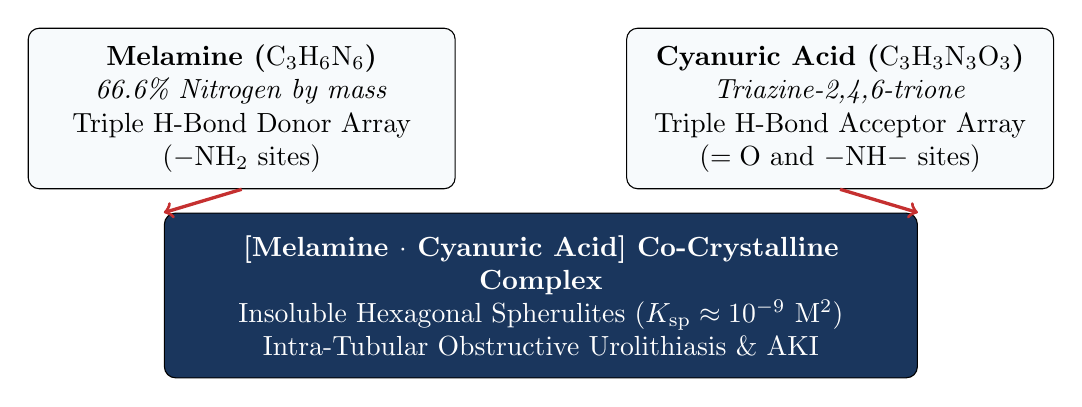
\begin{tikzpicture}[scale=0.95]
    % Melamine
    \node[draw, rectangle, rounded corners, fill=lightbg, inner sep=6pt] (mel) at (0,0) {
        \begin{minipage}{5cm}
        \centering
        \textbf{Melamine ($\mathrm{C_3H_6N_6}$)}\\
        \textit{66.6\% Nitrogen by mass}\\
        Triple H-Bond Donor Array\\
        ($-\mathrm{NH_2}$ sites)
        \end{minipage}
    };
    % Cyanuric Acid
    \node[draw, rectangle, rounded corners, fill=lightbg, inner sep=6pt] (cya) at (8,0) {
        \begin{minipage}{5cm}
        \centering
        \textbf{Cyanuric Acid ($\mathrm{C_3H_3N_3O_3}$)}\\
        \textit{Triazine-2,4,6-trione}\\
        Triple H-Bond Acceptor Array\\
        ($=\mathrm{O}$ and $-\mathrm{NH}-$ sites)
        \end{minipage}
    };
    % Complex
    \node[draw, rectangle, rounded corners, fill=primarynavy, text=white, inner sep=8pt] (complex) at (4,-2.5) {
        \begin{minipage}{9cm}
        \centering
        \textbf{[Melamine $\cdot$ Cyanuric Acid] Co-Crystalline Complex}\\
        Insoluble Hexagonal Spherulites ($K_{\text{sp}} \approx 10^{-9}\ \mathrm{M^2}$)\\
        Intra-Tubular Obstructive Urolithiasis \& AKI
        \end{minipage}
    };
    \draw[->, very thick, crimsonred] (mel.south) -- (complex.north west);
    \draw[->, very thick, crimsonred] (cya.south) -- (complex.north east);
\end{tikzpicture}
\end{figure}

Melamine ($\mathrm{C_3H_6N_6}$, 1,3,5-triazine-2,4,6-triamine) and its hydrolysis derivatives (\textbf{Ammeline}, \textbf{Ammelide}, \textbf{Cyanuric Acid}) are industrial precursors used in melamine-formaldehyde resin synthesis.
\begin{itemize}[leftmargin=*]
    \item \textbf{Analytical Exploitation:} Melamine contains $66.6\%$ nitrogen by mass. Standard Kjeldahl digestion breaks down all organic nitrogen into ammonium sulfate without distinguishing between protein peptide bonds ($-\mathrm{CONH}-$) and triazine ring nitrogen:
    $$\% \text{Apparent Protein} = \% \text{Total Nitrogen} \times 6.38$$
    Addition of only $0.1\text{ g}$ of melamine to $100\text{ g}$ of watered-down milk inflates the apparent crude protein reading by $0.425\%$.
\end{itemize}

\subsubsection{Ghee, Butter, Paneer, and Khoya}
\begin{itemize}[leftmargin=*]
    \item \textbf{Vanaspati (Hydrogenated Vegetable Oil) in Ghee:} Catalytic partial hydrogenation ($\mathrm{H_2 / Ni}$ catalyst at $180^\circ\text{C}$) of soybean, palm, or cottonseed oils converts unsaturated fatty acids into saturated and \textit{trans}-fatty acids (predominantly \textbf{elaidic acid}, $C_{18:1,\text{trans}-9}$).
    \begin{itemize}
        \item Pure cow ghee contains volatile short-chain fatty acids (butyric $C_4$, caproic $C_6$) and yields high \textbf{Reichert-Meissl (RM) values ($26-32$)}.
        \item Vanaspati contains long-chain $C_{16}-C_{18}$ fatty acids and yields an RM value $<1.0$.
    \end{itemize}
    \item \textbf{Animal Body Tallow / Lard in Ghee:} Body fats extracted from beef, mutton, or swine carcasses are characterized by saturated triglycerides rich in palmitic ($C_{16:0}$) and stearic ($C_{18:0}$) acids. They are distinguished from milk fat by stereospecific analysis of fatty acids at the $sn-2$ position and by differential scanning calorimetry (DSC).
    \item \textbf{Synthetic Paneer / Starch Adulteration:} Manufactured by coagulating a heated emulsion of skimmed milk powder, low-grade palm oil, and detergent with industrial sulfuric acid ($\mathrm{H_2SO_4}$) instead of food-grade citric or lactic acid. Starch and mashed potatoes are added to paneer and khoya to bind water and increase weight.
\end{itemize}

\subsection{Adulteration in Edible Oils and Fats}

\subsubsection{The *Argemone mexicana* Poisoning Cascade}
*Argemone mexicana* (Mexican prickly poppy) belongs to the family Papaveraceae. Its seeds resemble black mustard (*Brassica nigra*) seeds, but can be differentiated by microscopy:
\begin{itemize}
    \item \textbf{Mustard Seed Surface:} Smooth, finely reticulated, rounded.
    \item \textbf{Argemone Seed Surface:} Irregular, deeply pitted/wrinkled with a characteristic pointed apical beak.
\end{itemize}

\begin{hazardbox}{Biochemical Cascade of Sanguinarine Poisoning (Epidemic Dropsy)}
Argemone seed oil contains toxic quaternary benzophenanthridine alkaloids: \textbf{Sanguinarine} ($0.5-1.0\%$) and \textbf{Dihydrosanguinarine}.
\begin{enumerate}
    \item \textbf{Absorption and Target Binding:} Following intestinal absorption, sanguinarine selectively binds to the catalytic $\alpha$-subunit of the membrane-bound \textbf{$\mathrm{Na^+/K^+}$-ATPase} pump, competitively blocking the phosphorylation site.
    \item \textbf{Loss of Ionic Homeostasis:} Inhibition of active $\mathrm{Na^+}$ extrusion causes intracellular sodium and water accumulation, leading to generalized cellular edema.
    \item \textbf{Mitochondrial Uncoupling:} Sanguinarine uncouples mitochondrial oxidative phosphorylation by dissipating the proton gradient across the inner mitochondrial membrane, depleting cellular ATP.
    \item \textbf{Endothelial Hyper-Permeability:} It induces excessive synthesis and release of \textbf{Nitric Oxide ($\mathrm{NO}$)} via endothelial nitric oxide synthase (eNOS) activation. Elevated $\mathrm{NO}$ triggers widespread relaxation of vascular smooth muscle, extreme capillary vasodilation, and extravasation of fluid into interstitial tissues.
    \item \textbf{Clinical Syndrome (Epidemic Dropsy):}
    \begin{itemize}
        \item Severe bilateral dependent pitting edema of lower limbs.
        \item Cutaneous telangiectasia, erythema, and blanching rashes.
        \item Bilateral open-angle glaucoma due to blockage of the trabecular meshwork by hyper-dilated capillary loops.
        \item High-output congestive heart failure and pulmonary edema.
    \end{itemize}
\end{enumerate}
\end{hazardbox}

\subsubsection{Other Major Lipid Adulterations}
\begin{itemize}[leftmargin=*]
    \item \textbf{Mineral Oil / Liquid Paraffin:} Non-saponifiable petroleum hydrocarbon distillates added to mustard, sesame, and coconut oils. Identified by the \textbf{Holde's Saponification Test} (mineral oil remains insoluble and produces persistent turbidity upon dilution with water).
    \item \textbf{Castor Oil (*Ricinus communis*):} Contains \textbf{ricinoleic acid} ($12\text{-hydroxy-9-octadecenoic acid}$, up to $90\%$). Acts as a violent gastrointestinal irritant and cathartic purgative. Detected via thin-layer chromatography (TLC) of hydroxy fatty acids.
    \item \textbf{Cottonseed Oil in Edible Oils:} Contains toxic \textbf{Gossypol} (a polyphenolic dialdehyde that causes male infertility and hepatotoxicity) and cyclopropenoid fatty acids (\textbf{malvalic acid} and \textbf{sterculic acid}). Detected via the \textbf{Halphen Test} (reaction with sulfur in $\mathrm{CS_2}$/pyridine produces a deep red color).
    \item \textbf{Extra Virgin Olive Oil (EVOO) Fraud:} High-priced cold-pressed EVOO is diluted with refined pomace olive oil, solvent-extracted hazelnut oil, or soybean oil.
    \begin{itemize}
        \item \textit{Forensic Marker for Hazelnut Oil:} \textbf{Filbertone} ($(E)\text{-5-methylhept-2-en-4-one}$), detected via chiral GC-MS.
        \item \textit{Color Masking:} Old/deodorized oils are tinted with \textbf{Copper Chlorophyllin complexes (E141)} to simulate the fresh green appearance of polyphenol-rich EVOO.
    \end{itemize}
    \item \textbf{Thermally Degraded / Recycled Cooking Oil:} Repeated heating of cooking oils at frying temperatures ($>180^\circ\text{C}$) induces:
    \begin{enumerate}
        \item Hydrolysis generating Free Fatty Acids (FFA).
        \item Auto-oxidation generating lipid hydroperoxides, aldehydes (acrolein, 4-HNE), and ketones.
        \item Thermal polymerization forming cyclic monomeric, dimeric, and polymeric \textbf{Total Polar Compounds (TPC)}.
    \end{enumerate}
    \textbf{FSSAI Limit:} Maximum permitted TPC in frying oil is \textbf{$25\%$}. Cooking oil exceeding this limit is toxic and banned from further use.
\end{itemize}

\subsection{Adulteration in Spices and Condiments}

Spices command high market prices per unit weight, making them prime targets for illegal coloring, weighting, and substitution with exhausted residues.

\begin{center}
\begin{tabular}{@{}p{2.4cm} p{3.6cm} p{4.0cm} p{5.4cm}@{}}
\toprule
\textbf{Spice Matrix} & \textbf{Bioactive Target} & \textbf{Common Adulterants} & \textbf{Toxicology / Fraud Impact} \tabularnewline
\midrule
\textbf{Turmeric Powder} (*Curcuma longa*) & Curcuminoids ($3-6\%$ Curcumin, DMC, BDMC) & Metanil Yellow, Lead Chromate ($\mathrm{PbCrO_4}$), Starch, Chalk & Hepatotoxicity, microcytic lead anemia, saturnism, loss of curcumin potency \tabularnewline
\textbf{Chili Powder} (*Capsicum annuum*) & Capsaicinoids ($0.1-1.0\%$ Capsaicin, Dihydrocapsaicin) & Sudan I, II, III, IV, Rhodamine B, Brick powder, Red Lead ($\mathrm{Pb_3O_4}$) & IARC Group 3 carcinogenicity, DNA adducts, gastrointestinal mucosal ulceration \tabularnewline
\textbf{Black Pepper} (*Piper nigrum*) & Piperine ($4-9\%$ crystalline alkaloid) & Dried papaya seeds (*Carica papaya*), light berries, mineral oil & Carpine alkaloid gastrointestinal irritation, reduced piperine pungency \tabularnewline
\textbf{Coriander / Cumin} & Essential oils (Linalool, Cuminaldehyde) & Spent/exhausted seeds, dung powder, sawdust, Malachite Green & Pathogen vector (*Salmonella*), carcinogenic dye toxicity on fennel \tabularnewline
\textbf{Saffron} (*Crocus sativus*) & Crocin, Picrocrocin, Safranal & Safflower, dyed corn silk, shredded coconut, $\mathrm{BaSO_4}$/honey & Complete lack of bioactive crocetin, ingestion of toxic $\mathrm{Ba}^{2+}$ heavy metal salts \tabularnewline
\textbf{Asafoetida (Hing)} & Ferula gum resin (Ferulic acid, Umbelliferone) & Colophony (Pine) resin, soapstone, gypsum, wheat flour & Severe dyspepsia, lack of authentic organic sulfur/ferulic bioactives \tabularnewline
\textbf{Cinnamon} (*C. verum*) & Cinnamaldehyde ($>80\%$ of volatile oil) & Cassia bark (*Cinnamomum cassia*) & Cassia contains high levels of \textbf{Coumarin} ($>1\%$), a potent hepatotoxin and nephrotoxin \tabularnewline
\bottomrule
\end{tabular}
\end{center}

\subsection{Adulteration in Ice Cream, Frozen Desserts, and Dairy Emulsions}

Ice cream is a complex aerated multiphase emulsion-foam consisting of dispersed fat globules, ice crystals, and air cells suspended in a continuous freeze-concentrated aqueous sucrose-protein matrix.

\begin{itemize}[leftmargin=*]
    \item \textbf{Volatile Synthetic Aromas and Chemical Solvents:} Illicit manufacturers substitute authentic vanilla, fruit extracts, and dairy fats with hazardous industrial organic compounds:
    \begin{itemize}
        \item \textit{Pepper Oil and Synthetic Esters:} Added to impart intense artificial sharpness and aroma.
        \item \textit{Ethyl Acetate ($\mathrm{CH_3COOCH_2CH_3}$) and Butyraldehyde ($\mathrm{CH_3(CH_2)_2CHO}$):} Industrial solvent derivatives added to mimic fruity and creamy flavor profiles. Chronic exposure triggers mucosal necrosis, severe pulmonary inflammation, and central nervous system depression.
        \item \textit{Nitrate Salts ($\mathrm{KNO_3, NaNO_3}$):} Added to alter freezing characteristics and inhibit psychrotrophic bacterial growth. Nitrates undergo reduction to nitrites ($\mathrm{NO_2^-}$), inducing methemoglobinemia and reacting with secondary amines in the stomach to generate carcinogenic \textbf{$N$-nitrosamines}.
    \end{itemize}
    \item \textbf{Surfactants and Detergent Powders:} Commercial laundry detergents and alkyl benzene sulfonates are blended into synthetic ice cream mixes. They drastically reduce interfacial tension, generating excessive overrun (air incorporation $>120\%$) and creating an artificially creamy, stable foam that resists melting.
    \item \textbf{Slaughterhouse Carcass Glues and Non-Grade Gelatin:} Low-cost stabilizers formulated by boiling discarded animal carcass waste (tails, udders, nasal cartilage, tendons, and hooves). These unpurified animal glues carry massive microbial loads (*Bacillus cereus*, *Clostridium perfringens*), endotoxins, and heavy metal residues, causing severe chronic nephrotoxicity and gastrointestinal ulceration.
\end{itemize}

\subsection{Adulteration in Processed Condiments, Sauces, Jaggery, and Confectionery}

\begin{itemize}[leftmargin=*]
    \item \textbf{Tomato Sauces and Ketchup:} Genuine tomato solids (lycopene-rich tomato paste, minimum $25\%$ total soluble solids) are fraudulently substituted with:
    \begin{itemize}
        \item \textit{Pumpkin and Bottle Gourd Pulp:} Boiled vegetable starches used as bulking agents to increase viscosity and solid yield at minimal cost.
        \item \textit{Prohibited Coal-Tar Dyes:} Tinted with \textbf{Rhodamine B}, \textbf{Metanil Yellow}, and \textbf{Amaranth} to recreate the vibrant red color of ripe tomatoes.
        \item \textit{Excess Chemical Preservatives:} Overdoses of sodium benzoate ($\mathrm{C_6H_5COONa} > 2000\text{ ppm}$) and synthetic acetic acid to prevent rapid fermentation of the unhygienic vegetable pulp.
        \item \textit{Toxicology:} Chronic ingestion causes erosive gastritis, severe peptic ulceration, toxic chemical hepatitis, and systemic inflammation of vital organ systems.
    \end{itemize}
    \item \textbf{Jaggery (*Gur*):} Traditional unrefined non-centrifugal cane sugar is adulterated to artificially enhance brightness and shelf-life:
    \begin{itemize}
        \item \textit{Sodium Hydrosulfite ($\mathrm{Na_2S_2O_4}$, Hydrose / Rangolite):} Industrial reducing bleach added during cane juice boiling to decolorize dark molasses into a golden-yellow hue. Residual sulfur dioxide ($\mathrm{SO_2}$) induces violent asthmatic bronchospasms and allergic dermatitis.
        \item \textit{Washing Soda ($\mathrm{Na_2CO_3}$) and Chalk Powder ($\mathrm{CaCO_3}$):} Added to neutralize acidic, fermenting sugarcane juice and fraudulently inflate product weight. Ingestion leads to metabolic alkalosis, hypercalcemia, and renal calculi.
        \item \textit{Metanil Yellow Dye:} Imparts a durable golden-yellow color to low-grade jaggery cakes.
    \end{itemize}
    \item \textbf{Confectionery, Sweetmeats (*Mithai*), and Silver Leaf (*Vark*):}
    \begin{itemize}
        \item \textit{Non-Permitted Industrial Azo Dyes:} Widespread application of Metanil Yellow, Auramine, Rhodamine B, and Orange II in *laddoo*, *jalebi*, and *barfi*.
        \item \textit{Counterfeit Silver Foil (*Vark*):} Pure edible silver leaf ($99.9\%\ \mathrm{Ag}$, thickness $\approx 0.2\,\mu\text{m}$) is adulterated with or entirely replaced by \textbf{Toxic Aluminum Foil ($\mathrm{Al}$)}. Aluminum is a cumulative neurotoxin linked to microcytic anemia, neurofibrillary degeneration, and bone demineralization (osteomalacia).
    \end{itemize}
    \item \textbf{Jams, Jellies, and Fruit Juices:} Diluted with commercial high-fructose corn syrup (HFCS), invert sugar, molasses, synthetic carrageenan-gum blends, and artificial fruit esters, lacking authentic ascorbic acid and bioflavonoids.
\end{itemize}

\subsection{Artificial Forcing, Surface Dyes, and Chemical Preservatives in Produce, Fish, and Meat}

\subsubsection{Artificial Chemical Fruit Ripening (Calcium Carbide and Ethephon)}
Commercial traders artificially ripen immature fruits (mangoes, bananas, papayas) to capture early seasonal pricing:
\begin{formulabox}{Reaction Chemistry of Calcium Carbide ($\mathrm{CaC_2}$) Ripening}
Technical-grade calcium carbide reacts with ambient and surface moisture to release \textbf{Acetylene gas ($\mathrm{C_2H_2}$)}, a synthetic analog of the natural plant ripening hormone ethylene ($\mathrm{C_2H_4}$):
$$\mathrm{CaC_2 + 2\ H_2O \longrightarrow Ca(OH)_2 + C_2H_2\uparrow \quad (\Delta H = -127.9\text{ kJ/mol})}$$
\textbf{Toxic Industrial Contaminants:} Technical $\mathrm{CaC_2}$ contains inorganic impurities of \textbf{Calcium Arsenide ($\mathrm{Ca_3As_2}$)} and \textbf{Calcium Phosphide ($\mathrm{Ca_3P_2}$)}, which simultaneously generate highly lethal hydride gases:
$$\mathrm{Ca_3As_2 + 6\ H_2O \longrightarrow 3\ Ca(OH)_2 + 2\ AsH_3\uparrow \quad (Arsine\ Gas)}$$
$$\mathrm{Ca_3P_2 + 6\ H_2O \longrightarrow 3\ Ca(OH)_2 + 2\ PH_3\uparrow \quad (Phosphine\ Gas)}$$
\textbf{Clinical Toxicology:} Arsine and phosphine are potent cellular poisons. They cause non-immune intravascular hemolysis, acute tubular necrosis, cerebral edema, memory loss, intractable vomiting, and chronic carcinogenic transformation. Calcium carbide is \textbf{strictly prohibited under Regulation 2.3.5 of FSS (Prohibition and Restrictions on Sales) Regulations, 2011}.
\end{formulabox}

\subsubsection{Cosmetic Dyes and Hormonal Forcing in Fresh Vegetables}
\begin{itemize}[leftmargin=*]
    \item \textbf{Malachite Green Dipping:} Green vegetables (pointed gourd / *parwal*, okra / *bhindi*, green peas, green chilies) are dipped in solutions of \textbf{Malachite Green} (a toxic triphenylmethane dye) to impart a permanent, vivid emerald-green appearance.
    $$\mathrm{C_{23}H_{25}ClN_2 \quad (Bis(p\text{-dimethylaminophenyl})phenylmethylium\ chloride)}$$
    \textit{Pathology:} Malachite green is metabolically reduced in tissues to \textbf{leucomalachite green}, a persistent lipophilic metabolite that induces hepatic adenomas, thyroid follicular cysts, chromosomal aberrations, and multi-organ carcinogenesis (IARC classification).
    \item \textbf{Copper Sulphate ($\mathrm{CuSO_4}$) Greening:} Imparts a radiant green luster to processed peas and beans via copper-chlorophyll complexation. Excessive copper accumulation triggers Wilson's-like hepatolenticular degeneration, intravascular hemolysis, and acute kidney injury.
    \item \textbf{Oxytocin Hormonal Injection in Cucurbits:} Illicit parenteral administration of the peptide hormone \textbf{Oxytocin} into growing vines of pumpkins, bottle gourds, cucumbers, and watermelons. Oxytocin acts as a non-physiological growth stimulant, forcing rapid cellular elongation and massive water imbibition, causing fruits to double in size within 12--24 hours. Dietary absorption of residual hormones induces endocrine disruption, precocious puberty in young children, and female reproductive disorders.
    \item \textbf{Wax Coatings on Apples and Citrus:} Industrial morpholine-containing petroleum waxes and non-food grade paraffin applied to conceal age, prevent weight loss, and simulate fresh orchard harvest.
\end{itemize}

\subsubsection{Formalin Preservation in Seafood, Fish, and Meat}
\begin{hazardbox}{Chemistry and Pathophysiology of Formalin in Seafood}
\textbf{Chemical Agent:} \textbf{Formalin} ($37\text{--}40\%\ \text{w/v}$ aqueous solution of formaldehyde, $\mathrm{HCHO}$, stabilized with $10\text{--}15\%$ methanol).\\
\textbf{Fraudulent Intent:} Unscrupulous fish vendors dip freshly caught marine and freshwater fish, prawns, and dressed poultry in formalin baths to arrest autolytic decomposition and bacterial putrefaction during long-distance transportation without refrigeration. Formalin prevents the breakdown of fish proteins into volatile basic nitrogen (TVB-N) and suppresses the characteristic fishy odor of trimethylamine ($\mathrm{(CH_3)_3N}$), maintaining rigid flesh and bright red gills.\\
\textbf{Biochemical Cross-Linking Mechanism:} Formaldehyde is a powerful electrophilic cross-linking agent. It reacts with primary amino groups ($-\mathrm{NH_2}$) of lysine residues and guanidino groups of arginine on protein chains via methylene bridge formation:
$$\mathrm{Protein_1\text{-}NH_2 + HCHO + H_2N\text{-}Protein_2 \longrightarrow Protein_1\text{-}NH\text{-}CH_2\text{-}NH\text{-}Protein_2 + H_2O}$$
\textbf{Pathological Outcomes:}
\begin{enumerate}
    \item Rapid denaturation and cross-linking of mucosal lining in the esophagus and stomach, causing caustic chemical burns, severe erosive gastritis, and gastrointestinal perforation.
    \item In the liver and kidneys, formaldehyde is oxidized to \textbf{formic acid ($\mathrm{HCOOH}$)}, triggering severe metabolic acidosis, optic neuropathy, acute tubular necrosis, and anuria.
    \item Classified as a \textbf{Group 1 Proven Human Carcinogen} by IARC, directly implicated in nasopharyngeal carcinoma, sinonasal cancer, and myeloid leukemia.
\end{enumerate}
\end{hazardbox}

\subsection{Master Reference Matrix: Common Food Adulterants, Targets, and Clinical Consequences}

\begin{center}
\begin{tabular}{@{}p{3.2cm} p{5.0cm} p{7.6cm}@{}}
\toprule
\textbf{Food Matrix} & \textbf{Target Adulterant(s)} & \textbf{Biochemical Pathology \& Health Consequences} \tabularnewline
\midrule
\textbf{Milk \& Curd} & Unhygienic water, chalk, urea, detergent, starch, melamine & Diarrhea, acute gastroenteritis, nephrolithiasis, renal failure, bladder carcinoma \tabularnewline
\textbf{Ghee \& Butter} & Mashed potatoes, Vanaspati, animal body fats, lard, mineral oil & Coronary atherosclerosis, elevated LDL, gastrointestinal disturbances, loss of *danedar* grain \tabularnewline
\textbf{Edible Oils} & *Argemone* oil, mineral oil, Karanja oil, Castor oil, toxic dyes & Epidemic dropsy, glaucoma, cardiac arrest, cathartic purgation, gallbladder cancer \tabularnewline
\textbf{Food Grains} & Dust, pebbles, stones, weed seeds, ergot sclerotia, talc glaze & Intestinal obstruction, saturnism, ergotism gangrene, gastric mucosal abrasion \tabularnewline
\textbf{Pulses (Dhal)} & Metanil yellow, Lead chromate, Khesari dhal ($\beta$-ODAP) & Upper motor neuron lysis (neurolathyrism), microcytic lead anemia, testicular atrophy \tabularnewline
\textbf{Turmeric Powder} & Lead chromate ($\mathrm{PbCrO_4}$), Metanil yellow, sawdust, chalk & Lead encephalopathy, anemia, chronic saturnism, liver necrosis, DNA adducts \tabularnewline
\textbf{Chili Powder} & Red brick dust, Sudan dyes (I--IV), Rhodamine B, red lead & Severe gastric ulceration, IARC carcinogenic mutagenesis, heavy metal lead toxicity \tabularnewline
\textbf{Black Pepper} & Dried papaya seeds (*Carica papaya*), light berries & Gastric mucosal irritation, carpine alkaloid toxicity, liver disorders, indigestion \tabularnewline
\textbf{Mustard Seeds} & *Argemone mexicana* seeds & Epidemic dropsy, dependent pitting edema, glaucoma, myocardial failure \tabularnewline
\textbf{Cinnamon Sticks} & Cassia bark (*Cinnamomum cassia*) & Coumarin-induced hepatotoxicity, severe nephrotoxicity, oral mucosal ulcerations \tabularnewline
\textbf{Cumin Seeds} & Grass seeds colored with charcoal dust, spent cumin & Microbial gastroenteritis, lack of essential oils (cuminaldehyde), digestive cramps \tabularnewline
\textbf{Tea Leaves} & Exhausted/used tea leaves, artificial dyes, iron filings & Digestive disorders, liver damage, heavy metal intake, absence of tea polyphenols \tabularnewline
\textbf{Coffee Powder} & Chicory powder, roasted date/tamarind seed powder & Diarrhea, severe stomach cramps, flatulence, reduced stimulant caffeine potency \tabularnewline
\textbf{Sugar \& Jaggery} & Chalk powder, washing soda, urea, hydrose, metanil yellow & Chemical gastritis, metabolic alkalosis, renal failure, chronic carcinogenesis \tabularnewline
\textbf{Honey} & Molasses, dextrose, high-fructose corn syrup, invert syrup & Glycemic surges, metabolic syndrome, dental caries, loss of antibacterial inhibine \tabularnewline
\textbf{Ice Cream} & Detergent, pepper oil, ethyl acetate, butyraldehyde, animal glue & Chronic lung disorders, nephrotoxicity, myocardial damage, gastrointestinal inflammation \tabularnewline
\textbf{Tomato Sauces} & Pumpkin pulp, non-permitted coal tar dyes, artificial flavors & Erosive gastritis, toxic chemical hepatitis, systemic vital organ inflammation \tabularnewline
\textbf{Fruits (Fresh)} & Calcium carbide ($\mathrm{CaC_2}$ with arsine $\mathrm{AsH_3}$, phosphine $\mathrm{PH_3}$) & Neurotoxicity, memory loss, cerebral hypoxia, multi-organ carcinogenesis \tabularnewline
\textbf{Green Vegetables} & Malachite green, Copper sulphate ($\mathrm{CuSO_4}$), Oxytocin injection & Genotoxicity, thyroid follicular adenomas, endocrine disruption, early puberty \tabularnewline
\textbf{Fish \& Meat} & Formalin ($37\%$ aqueous formaldehyde $\mathrm{HCHO}$) & Caustic GI burns, severe metabolic acidosis, acute renal failure, Group 1 nasopharyngeal cancer \tabularnewline
\bottomrule
\end{tabular}
\end{center}

\newpage

% =============================================================================
% MODULE 3: METHODS OF FOOD ADULTERATION DETECTION
% =============================================================================
\section{Module 3: Methods of Food Adulteration Detection}

Food adulteration detection requires a comprehensive analytical arsenal spanning physical properties, wet chemical spot reactions, molecular biology, and advanced spectroscopic/chromatographic instrumentation.

\subsection{Advanced Instrumental Chemical Methods}

\subsubsection{Attenuated Total Reflectance FTIR (ATR-FTIR) Spectroscopy}
\begin{itemize}[leftmargin=*]
    \item \textbf{Physics of ATR Evanescent Wave:} Infrared radiation is directed through an internal reflection element (IRE) of high refractive index $n_1$ (e.g., Diamond $n_1=2.42$, Germanium $n_1=4.00$, ZnSe $n_1=2.40$) at an incidence angle $\theta$ exceeding the critical angle $\theta_c = \arcsin(n_2/n_1)$, where $n_2$ is the refractive index of the food sample ($n_2 \approx 1.3-1.5$).
    \item Total internal reflection generates an \textbf{evanescent electromagnetic wave} that penetrates into the sample:
    \begin{formulabox}{Depth of Evanescent Wave Penetration ($d_p$)}
    $$d_p = \frac{\lambda}{2\pi \sqrt{n_1^2 \sin^2\theta - n_2^2}}$$
    Where $\lambda$ is the infrared wavelength. For mid-IR radiation ($\lambda = 2.5-25\,\mu\text{m}$), $d_p \approx 0.5-2.0\,\mu\text{m}$.
    \end{formulabox}
    \item \textbf{Diagnostic Spectral Fingerprints:}
    \begin{itemize}
        \item \textit{Trans-Fatty Acids (Vanaspati in Ghee):} A sharp, isolated band at \textbf{$966\text{ cm}^{-1}$} corresponding to isolated trans $\mathrm{C=C}$ out-of-plane $(-\mathrm{CH}=\mathrm{CH}-)$ bending deformation (pure ghee exhibits no absorption at $966\text{ cm}^{-1}$).
        \item \textit{Melamine in Dairy Powders:} Sharp triazine ring in-plane quadrant stretch at \textbf{$810\text{ cm}^{-1}$} and ring skeletal stretches at \textbf{$1435\text{ cm}^{-1}$} and \textbf{$1550\text{ cm}^{-1}$}.
        \item \textit{Exogenous Sugars in Honey / Juices:} Carbohydrate $\mathrm{C-O}$ and $\mathrm{C-C}$ ring vibrational modes in the fingerprint region between \textbf{$950\text{ cm}^{-1}$ and $1150\text{ cm}^{-1}$}.
    \end{itemize}
\end{itemize}

\subsubsection{Surface-Enhanced Raman Scattering (SERS)}
\begin{itemize}[leftmargin=*]
    \item \textbf{Principle:} When molecules adsorb onto nanostructured noble metal surfaces (colloidal Gold or Silver nanoparticles, $\mathrm{Au/Ag}$ NPs), the Raman scattering cross-section is enhanced by factors of \textbf{$10^6\text{ to }10^8$} through two concurrent mechanisms:
    \begin{enumerate}
        \item \textit{Electromagnetic Enhancement:} Localized Surface Plasmon Resonance (LSPR) generated by incident laser excitation, creating intense electromagnetic ``hot-spots''.
        \item \textit{Chemical (Charge-Transfer) Enhancement:} Electronic charge transfer between the metal Fermi level and the lowest unoccupied molecular orbital (LUMO) of the analyte.
    \end{enumerate}
    \item \textbf{Applications:} Ultra-trace detection of \textbf{Melamine in milk ($<0.05\text{ ppm}$)}, \textbf{Rhodamine B}, \textbf{Sudan I in chili ($<0.1\text{ ppm}$)}, and pesticide residues (Chlorpyrifos, Malathion).
\end{itemize}

\subsubsection{\texorpdfstring{Stable Carbon Isotope Ratio Mass Spectrometry ($\delta^{13}\mathrm{C}$-IRMS)}{Stable Carbon Isotope Ratio Mass Spectrometry (delta-13C-IRMS)}}
Honey adulteration with inexpensive C4 plant sugars (High Fructose Corn Syrup / Cane Invert Syrup) is definitively detected by measuring stable carbon isotope ratios (${}^{13}\mathrm{C}/{}^{12}\mathrm{C}$).

\begin{formulabox}{Isotopic Fractionation Chemistry ($\delta^{13}\text{C}$)}
\textbf{1. Photosynthetic Pathways:}
\begin{itemize}
    \item \textbf{C3 Plants (Autochthonous Honey Flora):} Utilize the Calvin cycle; the enzyme \textbf{RuBisCO} discriminates strongly against ${}^{13}\mathrm{CO_2}$, resulting in depleted $\delta^{13}\text{C}$ values ranging from \textbf{$-23\permil\text{ to }-28\permil$}.
    \item \textbf{C4 Plants (Sugarcane, Maize / Corn):} Utilize the Hatch-Slack pathway; the enzyme \textbf{PEP Carboxylase} does not discriminate against ${}^{13}\mathrm{CO_2}$, resulting in enriched $\delta^{13}\text{C}$ values ranging from \textbf{$-10\permil\text{ to }-14\permil$}.
\end{itemize}
\textbf{2. Mathematical Definition:}
$$\delta^{13}\text{C}_{\text{sample}} (\permil) = \left[ \frac{\left(\frac{{}^{13}\text{C}}{{}^{12}\text{C}}\right)_{\text{sample}}}{\left(\frac{{}^{13}\text{C}}{{}^{12}\text{C}}\right)_{\text{VPDB standard}}} - 1 \right] \times 1000$$
Where $\text{VPDB} =$ Vienna Pee Dee Belemnite international standard.

\textbf{3. Internal Protein Standard Protocol (AOAC Official Method 998.12):}
Authentic pure honey contains trace natural protein ($0.1-0.5\%$) secreted by bees, which shares the identical $\delta^{13}\text{C}$ signature of the floral nectar:
$$\Delta \delta^{13}\text{C} = \delta^{13}\text{C}_{\text{protein}} - \delta^{13}\text{C}_{\text{whole honey}}$$
\textbf{Decision Thresholds:}
\begin{itemize}
    \item If $\Delta \delta^{13}\text{C} \ge -1.0\permil$, the honey is \textbf{pure / authentic}.
    \item If $\Delta \delta^{13}\text{C} < -1.0\permil$, the honey contains \textbf{exogenous C4 plant sugars}.
    \item $\% \text{ C4 Sugar Content} = \frac{\delta^{13}\text{C}_{\text{protein}} - \delta^{13}\text{C}_{\text{whole honey}}}{\delta^{13}\text{C}_{\text{protein}} - (-9.7)} \times 100$
    \item An apparent C4 sugar content \textbf{$>7\%$} constitutes regulatory adulteration.
\end{itemize}
\end{formulabox}

\subsubsection{Chromatographic Techniques: GC-MS and LC-MS/MS}
\begin{itemize}[leftmargin=*]
    \item \textbf{GC-FID / GC-MS for Fatty Acid Methyl Esters (FAME):}
    \begin{itemize}
        \item Triglycerides are transesterified with methanolic $\mathrm{KOH}$ or $\mathrm{BF_3-methanol}$ into volatile FAMEs:
        $$\mathrm{TAG + 3\ CH_3OH \xrightarrow{KOH / \Delta} 3\ R-COOCH_3 + Glycerol}$$
        \item Separated on a high-polarity capillary column (e.g., DB-WAX, 60 m $\times$ 0.25 mm ID, $0.25\,\mu\text{m}$ film).
        \item Differentiates butterfat from palm oil, beef tallow, and hydrogenated oils by calculating ratios of butyric acid ($C_{4:0}$), palmitic acid ($C_{16:0}$), and oleic/elaidic isomers ($C_{18:1,\text{cis}}$ vs $C_{18:1,\text{trans}}$).
    \end{itemize}
    \item \textbf{LC-MS/MS with Multiple Reaction Monitoring (MRM):}
    \begin{itemize}
        \item Ultra-high sensitivity quantification of non-volatile and thermally labile adulterants.
        \item Uses electrospray ionization (ESI) followed by collision-induced dissociation (CID) in a triple quadrupole mass spectrometer ($\mathrm{QqQ}$).
        \item *Sudan I Detection:* Precursor ion $[M+H]^+ = m/z\ 249.1 \to$ Diagnostic product ions $m/z\ 128.1$ and $m/z\ 93.1$.
        \item *Melamine Detection:* Precursor ion $[M+H]^+ = m/z\ 127.1 \to$ Product ions $m/z\ 85.1$ and $m/z\ 68.1$.
    \end{itemize}
\end{itemize}

\subsection{Standard Operating Protocols for Bench Wet Chemical Screening Tests}

\begin{protocolbox}{Protocol 1: Baudouin Test for Vanaspati in Pure Ghee / Butter}
\textbf{Principle:} Indian regulations require Vanaspati to contain $\ge 5\%$ sesame oil as an analytical marker. Sesame oil contains \textbf{Sesamol} (3,4-methylenedioxyphenol), which condenses with furfural in concentrated hydrochloric acid to form a resonance-stabilized quinoid cation complex.\\
\textbf{Reagents:} Concentrated Hydrochloric Acid ($\mathrm{HCl}$, sp. gr. 1.18); $2\%$ Furfural solution in distilled ethanol.\\
\textbf{Step-by-Step Procedure:}
\begin{enumerate}
    \item Take $5.0\text{ mL}$ of melted ghee sample in a clean, dry, glass-stoppered test tube.
    \item Add $5.0\text{ mL}$ of concentrated $\mathrm{HCl}$ and $0.4\text{ mL}$ of $2\%$ alcoholic furfural solution.
    \item Stopper the tube and shake vigorously for exactly 60 seconds.
    \item Allow the tube to stand undisturbed for 10 minutes to permit phase separation.
\end{enumerate}
\textbf{Observation \& Interpretation:}
\begin{itemize}
    \item \textit{Positive Result:} Development of a persistent \textbf{crimson-red or rose-red color} in the lower acid layer confirms the presence of sesame oil (and therefore Vanaspati).
    \item \textit{Negative Result:} Upper oily layer remains pale yellow; acid layer remains colorless or faint straw yellow.
\end{itemize}
\textbf{Limit of Detection (LOD):} Capable of detecting down to $1.0\%$ Vanaspati in pure ghee.
\end{protocolbox}

\begin{protocolbox}{Protocol 2: Nitric Acid and Ferric Chloride Tests for Argemone Oil in Mustard Oil}
\textbf{Principle:} Sanguinarine in *Argemone mexicana* oil forms a bright orange-red crystalline perchlorate or nitrate salt with concentrated nitric acid, and precipitates as a brownish-red complex with ferric chloride.\\
\textbf{Procedure A (Nitric Acid Test):}
\begin{enumerate}
    \item Take $5.0\text{ mL}$ of clear mustard oil sample in a test tube.
    \item Carefully add $5.0\text{ mL}$ of concentrated $\mathrm{HNO_3}$ down the side of the test tube.
    \item Shake gently and warm in a water bath at $60-70^\circ\text{C}$ for 10 minutes.
    \item \textit{Positive Result:} Development of a distinct \textbf{red-brown to crimson-orange color} at the oil-acid interface indicates Argemone oil contamination ($\text{LOD} \approx 0.1\%$).
\end{enumerate}
\textbf{Procedure B (Confirmatory Ferric Chloride Test):}
\begin{enumerate}
    \item Dissolve $10\text{ mL}$ of filtered oil in $15\text{ mL}$ petroleum ether.
    \item Extract three times with $5\text{ mL}$ portions of $1:1\ \mathrm{HCl}-\mathrm{H_2O}$.
    \item Evaporate the combined acid extract to dryness in a porcelain dish over a boiling water bath.
    \item Dissolve the residue in $1.0\text{ mL}$ of $0.1\,\mathrm{N}\ \mathrm{HCl}$ and add $1.0\text{ mL}$ of $2\%\ \mathrm{FeCl_3}$ reagent.
    \item \textit{Positive Result:} Formation of a reddish-brown precipitate with dark needle-like crystals under microscope confirms sanguinarine ($\text{LOD} \approx 0.01\%$).
\end{enumerate}
\end{protocolbox}

\begin{protocolbox}{Protocol 3: Halphen Test for Cottonseed Oil in Edible Oils}
\textbf{Principle:} Cottonseed oil contains cyclopropenoid fatty acids (\textbf{malvalic acid} and \textbf{sterculic acid}). When heated with sulfur dissolved in carbon disulfide and pyridine, the strained cyclopropene ring opens, reacting with sulfur to produce a stable cherry-red chromophore.\\
\textbf{Reagent Preparation:} Dissolve $1.0\text{ g}$ of precipitated sulfur in $100\text{ mL}$ of Carbon Disulfide ($\mathrm{CS_2}$); mix with $100\text{ mL}$ of analytical grade Pyridine.\\
\textbf{Procedure:}
\begin{enumerate}
    \item Pipette $5.0\text{ mL}$ of oil sample and $5.0\text{ mL}$ of Halphen reagent into a pressure-rated glass tube with a screw cap.
    \item Securely seal the tube and place it in a boiling saturated brine bath ($110-115^\circ\text{C}$) for 2 hours.
    \item \textit{Positive Result:} Development of a distinct \textbf{rose-red to cherry-red color} confirms cottonseed oil.
    \item \textit{LOD:} $0.5-1.0\%$ cottonseed oil.
\end{enumerate}
\end{protocolbox}

\begin{protocolbox}{Protocol 4: Fiehe's Test for Invert Sugar / Commercial Syrups in Honey}
\textbf{Principle:} Acid-catalyzed inversion of sucrose to produce commercial invert sugar syrup generates \textbf{Hydroxymethylfurfural (5-HMF)} as an acid-dehydration byproduct. Resorcinol in concentrated hydrochloric acid condenses with 5-HMF to yield a cherry-red condensation product.\\
\textbf{Reagents:} Resorcinol reagent ($1.0\text{ g}$ pure resorcinol dissolved in $100\text{ mL}$ concentrated $\mathrm{HCl}$); Diethyl Ether.\\
\textbf{Procedure:}
\begin{enumerate}
    \item Take $5.0\text{ g}$ of honey in a mortar and pestle; add $10\text{ mL}$ of diethyl ether and triturate thoroughly.
    \item Decant the clear ether layer into a white porcelain evaporating dish.
    \item Allow the ether to evaporate spontaneously at room temperature under a fume hood.
    \item Add 2 drops of freshly prepared resorcinol reagent to the dry residue.
    \item \textit{Positive Result:} Immediate appearance of a \textbf{cherry-red to deep scarlet color} that persists confirms acid-inverted sugar syrup.
\end{enumerate}
\end{protocolbox}

\begin{protocolbox}{Protocol 5: p-DMAB Spot Test for Exogenous Urea in Milk}
\textbf{Principle:} Exogenous urea reacts with $p$-dimethylaminobenzaldehyde ($p$-DMAB, Ehrlich's reagent) under acidic conditions to form a yellow-green Schiff base complex.\\
\textbf{Reagents:} $1.6\%\ (\text{w/v})\ p$-DMAB dissolved in ethyl alcohol containing $10\%\ (\text{v/v})$ concentrated $\mathrm{HCl}$.\\
\textbf{Procedure:}
\begin{enumerate}
    \item Take $5.0\text{ mL}$ of milk in a test tube.
    \item Add $5.0\text{ mL}$ of $1.6\%\ p$-DMAB reagent.
    \item Mix thoroughly and observe the color development within 2 minutes.
    \item \textit{Interpretation:}
    \begin{itemize}
        \item \textbf{Normal Pure Milk:} Distinct pale yellow or faint canary yellow color (due to physiological natural urea, $<0.05\%$).
        \item \textbf{Adulterated Milk:} Immediate development of a \textbf{deep yellow-green to dark emerald green color} indicates added synthetic urea ($>0.07\%$).
    \end{itemize}
\end{enumerate}
\end{protocolbox}

\begin{protocolbox}{Protocol 6: Detection of Neutralizers in Milk (Rosolic Acid Test)}
\textbf{Principle:} Neutralizers ($\mathrm{NaOH, Na_2CO_3, NaHCO_3}$) added to mask the acidity of spoiled milk shift the pH toward alkalinity. Rosolic acid (aurin) acts as a pH indicator, transitioning from yellow-brown to rose-pink at $\mathrm{pH} > 7.2$.\\
\textbf{Reagents:} $0.1\%\ (\text{w/v})$ Rosolic acid solution dissolved in $60\%\ (\text{v/v})$ ethanol.\\
\textbf{Procedure:}
\begin{enumerate}
    \item Take $5.0\text{ mL}$ of milk sample in a test tube.
    \item Add $5.0\text{ mL}$ of pure ethanol ($95\%$) and mix.
    \item Add 3--4 drops of $0.1\%$ rosolic acid indicator solution.
    \item \textit{Interpretation:}
    \begin{itemize}
        \item \textbf{Pure Milk:} Faint brownish-yellow or orange color.
        \item \textbf{Adulterated with Neutralizers:} Distinct \textbf{rose-red to crimson-pink color} confirms added alkaline carbonates or hydroxides.
    \end{itemize}
\end{enumerate}
\end{protocolbox}

\subsection{Physical and Biophysical Methods}

\subsubsection{Polarized Light Microscopy and Starch Birefringence}
\begin{itemize}[leftmargin=*]
    \item \textbf{Birefringence and Extinction Crosses:} Intact native starch granules possess a highly ordered radial crystalline arrangement of amylopectin side-chain double helices. Under a polarized light microscope with crossed nicols ($90^\circ$ polarization), starch granules exhibit optical anisotropy (birefringence) visible as a distinct \textbf{Maltese Cross (extinction cross)} centered at the hilum.
    \item \textbf{Morphological Differentiation of Starches:}
    \begin{center}
    \begin{tabular}{@{}p{2.8cm} p{4.2cm} p{8.4cm}@{}}
    \toprule
    \textbf{Starch Source} & \textbf{Granule Shape \& Size} & \textbf{Hilum \& Striation Characteristics} \tabularnewline
    \midrule
    \textbf{Potato Starch} & Large oval / egg-shaped ($50-100\,\mu\text{m}$) & Eccentric point hilum; distinct concentric growth rings \tabularnewline
    \textbf{Corn / Maize Starch} & Polyhedral / polygonal ($10-25\,\mu\text{m}$) & Central stellate (star-shaped) or split cleft hilum \tabularnewline
    \textbf{Wheat Starch} & Bimodal: large lenticular ($20-35\,\mu\text{m}$) \& small spherical ($2-8\,\mu\text{m}$) & Central circular hilum; faint concentric striations \tabularnewline
    \textbf{Rice Starch} & Very small angular polyhedral ($2-7\,\mu\text{m}$) & Compound granule clusters; non-distinct hilum \tabularnewline
    \textbf{Chickpea (Besan)} & Oval to reniform ($15-30\,\mu\text{m}$) & Prominent elongated longitudinal cleft; distinct Maltese cross \tabularnewline
    \bottomrule
    \end{tabular}
    \end{center}
    \item \textbf{Thermal Gelatinization Loss:} Heating starch above its gelatinization temperature ($65-75^\circ\text{C}$) disrupts the crystalline amylopectin structure, causing irreversible swelling and total loss of birefringence and Maltese crosses.
\end{itemize}

\subsubsection{Hortvet Freezing Point Cryoscopy of Milk}
The freezing point of milk is its most constant physical property, maintained in tight osmotic equilibrium with maternal blood serum by dissolved lactose and mineral salts ($\mathrm{K^+, Na^+, Cl^-}$).

\begin{formulabox}{Freezing Point Cryoscopy Formulation}
Pure bovine milk has a freezing point ($T_f$) of \textbf{$-0.525^\circ\text{C}$ to $-0.550^\circ\text{C}$} ($540-550\text{ m}^\circ\text{H}$ on the Hortvet scale).
Addition of water dilutes ionic solutes, shifting $T_f$ toward $0.000^\circ\text{C}$ in accordance with \textbf{Raoult's Law of Freezing Point Depression}:
$$\Delta T_f = K_f \cdot m \cdot i$$
Where $K_f = 1.86^\circ\text{C}\cdot\text{kg/mol}$ is the cryoscopic constant of water.

\textbf{Percentage of Added Water Calculation (AOAC Official Method 922.08):}
$$\% \text{ Added Water} = \frac{T_{f,\text{base}} - T_{f,\text{sample}}}{T_{f,\text{base}}} \times 100$$
Where regulatory baseline $T_{f,\text{base}} = -0.525^\circ\text{C}$.
\end{formulabox}

\subsubsection{Differential Scanning Calorimetry (DSC)}
\begin{itemize}[leftmargin=*]
    \item \textbf{Principle:} DSC measures the differential heat flow into a sample relative to an inert reference pan as a function of temperature under controlled heating/cooling cycles:
    $$\frac{dH}{dt} = C_p \frac{dT}{dt} + f(T, t)$$
    \item \textbf{Application in Lipid Adulteration:} Pure milk fat exhibits three characteristic endothermic melting peaks corresponding to low-melting ($\approx -10^\circ\text{C}$), medium-melting ($\approx 15^\circ\text{C}$), and high-melting ($\approx 35^\circ\text{C}$) triacylglycerol fractions.
    \begin{itemize}
        \item Adulteration with \textbf{Vanaspati / Palm Stearin} introduces an anomalous endothermic melting peak at \textbf{$45-55^\circ\text{C}$}.
        \item Adulteration with \textbf{Lard / Tallow} alters the polymorphic crystallization transition enthalpy ($\Delta H_{\text{crys}}$).
    \end{itemize}
\end{itemize}

\subsection{Biological and Molecular Methods}

\subsubsection{Multiplex Real-Time PCR for Meat Speciation}
DNA-based detection relies on the high stability of double-stranded DNA against thermal processing and rendering compared to labile proteins.

\begin{mechanismbox}{TaqMan Real-Time qPCR Speciation Architecture}
\textbf{1. Target Gene Selection:} High copy-number \textbf{mitochondrial DNA (mtDNA)} genes:
\begin{itemize}
    \item \textit{Cytochrome b (cyt b)}
    \item \textit{Cytochrome c Oxidase Subunit I (COI)}
    \item \textit{Mitochondrial 12S / 16S rRNA}
    \item \textit{Displacement Loop (D-loop)}
\end{itemize}
\textbf{Mitochondrial Advantage:} Each somatic muscle cell contains 1,000--10,000 copies of mtDNA compared to only 2 copies of nuclear DNA, allowing detection even in cooked or canned meats down to \textbf{$0.01\%\ (\text{w/w})$}.

\textbf{2. TaqMan Fluorogenic Dual-Labeled Probe Chemistry:}
During the annealing step, a sequence-specific fluorogenic probe anneals to the template DNA between forward and reverse primers. The probe carries a 5'-reporter dye (e.g., $\mathrm{FAM, VIC, HEX}$) and a 3'-quencher dye (e.g., $\mathrm{TAMRA, BHQ-1}$):
\begin{enumerate}
    \item In the intact probe, the quencher suppresses fluorescence via \textbf{Förster Resonance Energy Transfer (FRET)}.
    \item During the extension cycle, thermostable \textit{Taq} DNA Polymerase advances along the template. Its \textbf{$5' \to 3'$ exonuclease activity} hydrolyzes the hybridized probe.
    \item Cleavage physically separates the reporter fluorophore from the quencher, generating a fluorescence signal proportional to the accumulated amplicon:
    $$\Delta R_n = R_n^+ - R_n^-$$
\end{enumerate}
\textbf{3. Multiplexing Capability:} By utilizing distinct fluorophores on species-specific probes ($\mathrm{FAM}$ for Bovine, $\mathrm{VIC}$ for Equine, $\mathrm{HEX}$ for Porcine, $\mathrm{Cy5}$ for Ovine), a single multiplex reaction identifies all target species simultaneously.
\end{mechanismbox}

\subsubsection{Enzyme-Linked Immunosorbent Assay (ELISA)}
\begin{itemize}[leftmargin=*]
    \item \textbf{Sandwich ELISA Protocol for Protein Adulterants:}
    \begin{enumerate}
        \item Microtiter wells coated with primary capture monoclonal antibody ($\mathrm{mAb_1}$) specific to target antigen (e.g., Bovine $\beta$-lactoglobulin).
        \item Sample extract added; target antigen binds specifically to immobilized $\mathrm{mAb_1}$.
        \item Unbound matter removed by washing with PBST.
        \item Enzyme-conjugated secondary antibody ($\mathrm{mAb_2}$-HRP, Horseradish Peroxidase) added, forming an antibody-antigen-antibody sandwich.
        \item Chromogenic substrate ($3,3',5,5'\text{-tetramethylbenzidine}$, TMB) added:
        $$\mathrm{TMB_{\text{reduced}} (Colorless) + H_2O_2 \xrightarrow{HRP} TMB_{\text{oxidized}} (Blue)}$$
        $$\mathrm{TMB_{\text{oxidized}} \xrightarrow{H_2SO_4} Diimine\ (Yellow,\ \lambda = 450\text{ nm})}$$
        \item Absorbance at $450\text{ nm}$ is measured on a microplate spectrophotometer; absorbance is directly proportional to antigen concentration.
    \end{enumerate}
\end{itemize}

\newpage

% =============================================================================
% MODULE 4: QUALITY ASSESSMENT PARAMETERS
% =============================================================================
\section{Module 4: Quality Assessment Parameters}

Food quality assurance requires comprehensive analysis of sensory attributes, proximate composition, lipid stability indices, and microbiological safety.

\subsection{Sensory and Organoleptic Evaluation (ISO 8589 Standards)}

\subsubsection{Sensory Booth Environment and Experimental Controls}
Sensory analysis uses human senses under controlled conditions conforming to \textbf{ISO 8589}:
\begin{itemize}[leftmargin=*]
    \item \textbf{Testing Booths:} Individual partitioned booths isolated from noise, extraneous cooking odors, and visual distractions; maintained at $21\pm 2^\circ\text{C}$ and $50\pm 5\%$ relative humidity.
    \item \textbf{Lighting Controls:} Standard D65 daylight-equivalent lighting ($6500\text{ K}$); red or green monochromatic lighting is employed to mask color differences during pure flavor discrimination tests.
    \item \textbf{Sample Presentation:} Samples served in odor-free glass containers labeled with \textbf{3-digit random numbers} generated from statistical tables.
\end{itemize}

\subsubsection{Sensory Testing Methodologies and Statistical Principles}

\begin{center}
\begin{tabular}{@{}p{3.0cm} p{4.0cm} p{9.0cm}@{}}
\toprule
\textbf{Test Category} & \textbf{Methodology} & \textbf{Statistical Principle and Hypothesis Testing} \tabularnewline
\midrule
\textbf{Triangle Test} (ISO 4120) & Panelists receive 3 coded samples simultaneously (2 controls, 1 treated). Must identify the odd sample. & Guessing probability $p = 1/3$. Statistically evaluated via binomial distribution:
$$P(X \ge k) = \sum_{x=k}^{n} \binom{n}{x} \left(\frac{1}{3}\right)^x \left(\frac{2}{3}\right)^{n-x}$$
Where $n =$ number of panelists, $k =$ correct responses. Evaluated at $\alpha = 0.05$ or $0.01$. \tabularnewline
\textbf{Duo-Trio Test} (ISO 10399) & Panelists receive a reference sample ($R$) followed by two coded samples; must identify which matches $R$. & Guessing probability $p = 1/2$. Lower statistical power than Triangle test; preferred for highly fatiguing taste matrices. \tabularnewline
\textbf{Quantitative Descriptive Analysis (QDA)} & Trained descriptive panel (10--12 experts) identifies, defines, and rates specific flavor, texture, and aroma descriptors on continuous 15-cm line scales. & Data normalized by ANOVA; results plotted as multivariate \textbf{radar / spider web sensory profiles}; analyzed via Principal Component Analysis (PCA). \tabularnewline
\textbf{9-Point Hedonic Scale} (Peryam \& Pilgrim) & Untrained consumer panel ($n \ge 60-100$) rates affective acceptance on a 9-point anchored bipolar scale. & Scale ranges from 1 (``Dislike Extremely'') to 5 (``Neither Like nor Dislike'') to 9 (``Like Extremely''). Data evaluated via ANOVA and Tukey's HSD test. \tabularnewline
\bottomrule
\end{tabular}
\end{center}

\subsection{Nutritional Proximate Chemical Analysis (Weende System)}

\subsubsection{Moisture Determination and Karl Fischer Titration}
\begin{itemize}[leftmargin=*]
    \item \textbf{Thermal Oven Drying ($105^\circ\text{C}$):} Sample dried to constant mass ($\Delta m < 0.001\text{ g}$). For high-sugar products (honey, fruit juices), \textbf{vacuum oven drying at $70^\circ\text{C}$ ($\le 50\text{ mmHg}$)} is mandated to prevent thermal caramelization and Maillard browning reactions.
    \item \textbf{Karl Fischer Volumetric / Coulometric Titration:} For trace water in edible oils, dried milk powder, and confectionery.
    \begin{formulabox}{Karl Fischer Reaction Stoichiometry}
    $$\mathrm{I_2 + SO_2 + 3\ RN + CH_3OH + H_2O \longrightarrow 2\ (RNH^+)I^- + (RNH^+)SO_4CH_3^-}$$
    Where $\mathrm{RN}$ is an organic base (imidazole or pyridine). In coulometric KF, iodine ($\mathrm{I_2}$) is generated electrochemically at the platinum anode:
    $$2\ \mathrm{I^- \longrightarrow I_2 + 2\ e^-}$$
    According to Faraday's Law, $1\text{ mole of }\mathrm{I_2}\ (2\times 96{,}485\text{ C})$ corresponds to $1\text{ mole of }\mathrm{H_2O}\ (18.015\text{ g})$.
    \end{formulabox}
\end{itemize}

\subsubsection{Crude Protein Determination: The Kjeldahl Method}

\begin{formulabox}{Chemical Reactions and Calculations of the Kjeldahl Method}
\textbf{Step 1: Acid Digestion}
Sample is boiled with concentrated $\mathrm{H_2SO_4}$ ($98\%$) in the presence of catalyst ($\mathrm{CuSO_4}$ or $\mathrm{TiO_2}$) and boiling point elevator ($\mathrm{K_2SO_4}$, elevating $T$ to $370-400^\circ\text{C}$):
$$\text{Organic Nitrogen} + \mathrm{H_2SO_4} \xrightarrow{\Delta,\ \mathrm{CuSO_4/K_2SO_4}} \mathrm{(NH_4)_2SO_4 + CO_2\uparrow + SO_2\uparrow + H_2O}$$

\textbf{Step 2: Neutralization and Steam Distillation}
Digest is basified with excess concentrated ($40\%\ \text{w/v}$) $\mathrm{NaOH}$ to liberate ammonia gas:
$$\mathrm{(NH_4)_2SO_4 + 2\ NaOH \longrightarrow 2\ NH_3\uparrow + Na_2SO_4 + 2\ H_2O}$$
Liberated $\mathrm{NH_3}$ is steam-distilled into a trapping solution of $4\%$ boric acid containing Tashiro's indicator (Methyl Red + Methylene Blue):
$$\mathrm{NH_3 + H_3BO_3 \longrightarrow NH_4^+ + H_2BO_3^- \quad (Borate\ Complex)}$$

\textbf{Step 3: Acidimetric Titration}
The dihydrogen borate ion is titrated with standardized hydrochloric acid ($0.1\,\mathrm{N}\ \mathrm{HCl}$):
$$\mathrm{H_2BO_3^- + H^+ \longrightarrow H_3BO_3}$$

\textbf{Mathematical Calculation:}
$$\% \text{ Nitrogen (N)} = \frac{(V_{\text{sample}} - V_{\text{blank}}) \times N_{\mathrm{HCl}} \times 14.007}{\text{Sample Weight (g)} \times 10}$$
$$\% \text{ Crude Protein} = \% \text{ Nitrogen} \times F_{\text{factor}}$$
Where empirical conversion factors $F$ are:
\begin{itemize}
    \item $F = 6.38$ for Whole Milk, Dairy Products, and Casein.
    \item $F = 5.70$ for Wheat Flours, Bread, and Pasta.
    \item $F = 5.95$ for Rice and Rice Products.
    \item $F = 5.30$ for Soybeans and Legumes.
    \item $F = 6.25$ for Meat, Eggs, Fish, and General Mixed Foods.
\end{itemize}
\end{formulabox}

\subsubsection{Crude Fat, Ash, and Carbohydrate Profiling}
\begin{itemize}[leftmargin=*]
    \item \textbf{Crude Fat (Soxhlet Continuous Extraction):} Moisture-free ground sample is extracted in a Soxhlet apparatus using non-polar petroleum ether (b.p. $40-60^\circ\text{C}$) or diethyl ether for 6--16 hours. For dairy products, the \textbf{Mojonnier Method} (acid hydrolysis with concentrated $\mathrm{HCl}$ followed by extraction with ethanol, ethyl ether, and petroleum ether) is used to liberate fat bound to proteins.
    \item \textbf{Total Ash:} Incineration of organic matrix in a muffle furnace at \textbf{$550^\circ\text{C} \pm 20^\circ\text{C}$} until light gray, carbon-free inorganic ash remains.
    \item \textbf{Acid Insoluble Ash (AIA):} Total ash is boiled in $10\%\ (\text{v/v})\ \mathrm{HCl}$, filtered through ashless Whatman 42 filter paper, washed with hot water, and re-incinerated at $550^\circ\text{C}$. AIA measures extraneous silica, sand, dirt, and talc contamination.
    \item \textbf{Available Carbohydrates (By Difference):}
    $$\% \text{ Carbohydrates} = 100 - [\% \text{Moisture} + \% \text{Crude Protein} + \% \text{Crude Fat} + \% \text{Ash} + \% \text{Crude Fiber}]$$
    \item \textbf{Caloric Energy Calculation (Atwater Physiological Factors):}
    $$\text{Energy (kcal/100 g)} = 4 \times (\% \text{Protein}) + 9 \times (\% \text{Fat}) + 4 \times (\% \text{Carbohydrate})$$
\end{itemize}

\subsection{Physicochemical Indices of Fats and Oils}

\begin{formulabox}{Essential Physicochemical Lipid Formulas}
\textbf{1. Acid Value (AV) and Free Fatty Acids (FFA):}
Measures the quantity of free fatty acids liberated by hydrolytic cleavage of triglyceride ester bonds:
$$\text{Acid Value (mg KOH/g)} = \frac{V_{\mathrm{KOH}} \times N_{\mathrm{KOH}} \times 56.11}{\text{Sample Weight (g)}}$$
$$\% \text{ FFA (as Oleic Acid, MW 282.46)} = \frac{\text{Acid Value}}{1.99} = \frac{V_{\mathrm{KOH}} \times N_{\mathrm{KOH}} \times 28.2}{\text{Sample Weight (g)}}$$

\textbf{2. Saponification Value (SV):}
Milligrams of $\mathrm{KOH}$ required to completely saponify $1.0\text{ g}$ of fat. Inversely proportional to the mean molecular weight (chain length) of fatty acids:
$$\text{Saponification Value} = \frac{(V_{\text{blank}} - V_{\text{sample}}) \times N_{\mathrm{KOH}} \times 56.11}{\text{Sample Weight (g)}}$$
$$\text{Mean Molecular Weight of Triglyceride} = \frac{3 \times 56.11 \times 1000}{\text{Saponification Value}}$$

\textbf{3. Iodine Value (IV, Wijs Method):}
Grams of halogen (expressed as iodine) absorbed by $100\text{ g}$ of fat. Direct quantitative measure of carbon-carbon double bond ($\mathrm{C=C}$) unsaturation:
$$\mathrm{-CH=CH- + ICl \longrightarrow -CH(I)-CH(Cl)-}$$
$$\mathrm{Excess\ ICl + 2\ I^- \longrightarrow I_2 + Cl^-}$$
$$\mathrm{I_2 + 2\ S_2O_3^{2-} \longrightarrow 2\ I^- + S_4O_6^{2-}}$$
$$\text{Iodine Value} = \frac{(V_{\text{blank}} - V_{\text{sample}}) \times N_{\mathrm{Na_2S_2O_3}} \times 12.69}{\text{Sample Weight (g)}}$$

\textbf{4. Peroxide Value (PV):}
Quantifies primary lipid oxidation products (lipid hydroperoxides, $\mathrm{ROOH}$) via iodometric titration:
$$\mathrm{ROOH + 2\ I^- + 2\ H^+ \longrightarrow ROH + I_2 + H_2O}$$
$$\mathrm{I_2 + 2\ S_2O_3^{2-} \longrightarrow 2\ I^- + S_4O_6^{2-}}$$
$$\text{Peroxide Value (meq }\mathrm{O_2}\text{/kg fat)} = \frac{(V_{\text{sample}} - V_{\text{blank}}) \times N_{\mathrm{Na_2S_2O_3}} \times 1000}{\text{Sample Weight (g)}}$$

\textbf{5. $p$-Anisidine Value ($p$-AV) and Totox Value:}
$p$-Anisidine reacts with secondary oxidation products ($\alpha,\beta$-unsaturated aldehydes, predominantly 2-alkenals and 2,4-dienals) in glacial acetic acid to form a yellow Schiff base measured spectrophotometrically at \textbf{$\lambda = 350\text{ nm}$}:
$$p\text{-AV} = \frac{25 \times (1.2 \times A_{\text{reacted}} - A_{\text{blank}})}{\text{Sample Weight (g)}}$$
$$\mathbf{Totox\ Value} = 2 \times \text{Peroxide Value (PV)} + p\text{-Anisidine Value (}p\text{-AV)}$$
\end{formulabox}

\subsection{Microbiological Quality and Safety Criteria}

\begin{center}
\begin{tabular}{@{}p{3.0cm} p{3.8cm} p{3.8cm} p{4.8cm}@{}}
\toprule
\textbf{Microorganism} & \textbf{Selective Media} & \textbf{Growth Conditions} & \textbf{Health \& Safety Impact} \tabularnewline
\midrule
\textbf{Total Viable Count (TVC)} & Plate Count Agar (PCA) & $30^\circ\text{C}$ or $37^\circ\text{C}$ for $48\pm 2\text{ h}$; all visible colonies counted & Indicator of overall hygiene, sanitary handling, and shelf-life \tabularnewline
\textbf{Coliforms / \textit{E. coli}} & Violet Red Bile Agar (VRBA) / Eosin Methylene Blue (EMB) & $37^\circ\text{C} / 44.5^\circ\text{C}$ for $24\text{ h}$; green metallic sheen on EMB & Indicator of fecal contamination and sanitation failure \tabularnewline
\textbf{\textit{Salmonella enterica}} & Xylose Lysine Deoxycholate (XLD) Agar & $37^\circ\text{C}$ for $24\text{ h}$; pink-red colonies with black centers ($\mathrm{H_2S}$) & Zero-tolerance enteric pathogen; causes salmonellosis and enteric fever \tabularnewline
\textbf{\textit{Staphylococcus aureus}} & Baird-Parker Agar with Egg Yolk Tellurite & $37^\circ\text{C}$ for $24-48\text{ h}$; shiny black colonies with clear halo & Produces heat-stable staphylococcal enterotoxins (A, B, C, D) \tabularnewline
\textbf{\textit{Listeria monocytogenes}} & Oxford Agar / PALCAM Agar & $30-37^\circ\text{C}$; psychrotrophic (grows at $4^\circ\text{C}$); black halo & Invasive listeriosis, septicemia, meningitis, maternal-fetal death \tabularnewline
\textbf{Yeast and Molds} & Dichloran Rose Bengal Chloramphenicol (DRBC) & $25^\circ\text{C}$ for 5 days; filamentous or mucoid colonies & Food spoilage; synthesis of mycotoxins (Aflatoxins, Ochratoxin A) \tabularnewline
\bottomrule
\end{tabular}
\end{center}

\newpage

% =============================================================================
% MODULE 5: FOOD SAFETY REGULATIONS AND STANDARDS
% =============================================================================
\section{Module 5: Food Safety Regulations and Standards}

Food safety governance relies on an integrated architecture of international normative bodies, statutory national authorities, proactive quality management systems, and legal compliance frameworks.

\subsection{International Regulatory Architecture and Treaties}

\begin{center}
\begin{tabular}{@{}p{3.2cm} p{4.2cm} p{8.6cm}@{}}
\toprule
\textbf{Regulatory Authority} & \textbf{Governance \& Mandate} & \textbf{Core Statutory Frameworks \& Global Impact} \tabularnewline
\midrule
\textbf{Codex Alimentarius Commission (CAC)} & Joint FAO/WHO intergovernmental body established in 1963; 189 member states. & Publishes the \textbf{Codex Alimentarius} (international food code), commodity standards, Maximum Residue Limits (MRLs) for pesticides/veterinary drugs, and the General Standard for Food Additives (GSFA). Recognized by the World Trade Organization (WTO) under the \textbf{SPS Agreement} and \textbf{TBT Agreement} as the international benchmark for resolving trade disputes. \tabularnewline
\textbf{US Food and Drug Administration (FDA)} & United States federal regulatory agency under the Department of Health and Human Services (HHS). & Enforces the \textbf{Food Safety Modernization Act (FSMA, 2011)}, shifting focus from reactive response to proactive prevention via \textbf{Hazard Analysis and Risk-Based Preventive Controls (HARPC)}, Foreign Supplier Verification Programs (FSVP), and Import Alerts. \tabularnewline
\textbf{European Food Safety Authority (EFSA)} & Independent scientific risk assessment agency of the European Union. & Governed by \textbf{Regulation (EC) No 178/2002} (General Food Law). Operates the Rapid Alert System for Food and Feed (\textbf{RASFF}) for border rejections, public health warnings, and traceability recalls across EU member states. \tabularnewline
\textbf{International Organization for Standardization (ISO)} & Global non-governmental federation of national standard bodies. & Develops international consensus management standards, notably \textbf{ISO 22000:2018} (Food Safety Management Systems) and \textbf{ISO/IEC 17025:2017} (Testing and Calibration Laboratories). \tabularnewline
\bottomrule
\end{tabular}
\end{center}

\subsection{National Regulatory Authority: FSSAI and the FSSA 2006}

The \textbf{Food Safety and Standards Act (FSSA), 2006} unified and repealed eight fragmented, multi-departmental legacy food orders in India:

\begin{defbox}{Legislative Consolidation under FSSA 2006}
The FSSA 2006 repealed and superseded:
\begin{enumerate}[label=(\roman*)]
    \item Prevention of Food Adulteration Act (PFA), 1954;
    \item Fruit Products Order (FPO), 1955;
    \item Meat Food Products Order (MFPO), 1973;
    \item Vegetable Oil Products (Control) Order, 1947;
    \item Edible Oils Packaging (Regulation) Order, 1998;
    \item Solvent Extracted Oil, De-oiled Meal and Edible Flour Control Order, 1967;
    \item Milk and Milk Products Order (MMPO), 1992;
    \item Any other order under the Essential Commodities Act, 1955 relating to food.
\end{enumerate}
\end{defbox}

\subsubsection{Key FSSAI Regulations and Statutory Initiatives}
\begin{itemize}[leftmargin=*]
    \item \textbf{FSS (Licensing and Registration of Food Businesses) Regulations, 2011:}
    \begin{itemize}
        \item *Registration:* Petty food business operators (annual turnover $<$ Rs.~12 Lakhs).
        \item *State License:* Medium food businesses (annual turnover Rs.~12 Lakhs to Rs.~20 Crores).
        \item *Central License:* Large manufacturers, 100\% Export Oriented Units, importers, operations at ports/airports, or annual turnover $>$ Rs.~20 Crores.
    \end{itemize}
    \item \textbf{FSS (Packaging) Regulations, 2018:} Prohibits recycled plastics and printed newspaper wrapping for food contact; specifies overall migration limits ($60\text{ mg/kg}$ or $10\text{ mg/dm}^2$) and specific migration limits (SML) for heavy metals and phthalates.
    \item \textbf{FSS (Labelling and Display) Regulations, 2020:} Mandates list of ingredients in descending order of weight, nutritional information per $100\text{ g}$ or per serve, mandatory allergen declarations, vegetarian/non-vegetarian logos, Date of Minimum Durability (``Best Before'' vs ``Expiry Date''), and batch lot numbers.
    \item \textbf{DART Initiative (Detect Adulteration with Rapid Test):} A manual of 50+ rapid household chemical and physical screening tests published by FSSAI for consumer awareness.
    \item \textbf{Food Safety on Wheels (FSW):} Mobile analytical testing laboratories equipped with spectrophotometers, refractometers, and milk analyzers deployed across India for on-the-spot screening.
\end{itemize}

\subsection{Food Safety Management Systems: HACCP and ISO 22000}

\begin{protocolbox}{The 7 Principles of HACCP (Hazard Analysis and Critical Control Points)}
\begin{enumerate}[leftmargin=*]
    \item \textbf{Principle 1: Conduct a Hazard Analysis} -- Identify biological (pathogens), chemical (mycotoxins, pesticide residues, allergens, adulterants), and physical (glass, metal fragments) hazards at each step of the process flow.
    \item \textbf{Principle 2: Determine Critical Control Points (CCPs)} -- Apply the \textbf{Codex HACCP Decision Tree} to identify process steps essential to prevent, eliminate, or reduce a food safety hazard to an acceptable level.
    \item \textbf{Principle 3: Establish Critical Limits} -- Establish validated minimum/maximum parameters for each CCP (e.g., High-Temperature Short-Time pasteurization: temperature $\ge 71.7^\circ\text{C}$ for holding time $\ge 15\text{ seconds}$).
    \item \textbf{Principle 4: Establish Monitoring Procedures} -- Implement scheduled, continuous measurements to ensure the CCP remains within critical limits (e.g., automated temperature chart recorders and flow diverter valves).
    \item \textbf{Principle 5: Establish Corrective Actions} -- Define predetermined protocols to execute when monitoring indicates a deviation from a critical limit (e.g., automatically divert under-pasteurized milk back to raw balance tank; isolate and quarantine affected batch).
    \item \textbf{Principle 6: Establish Verification Procedures} -- Conduct activities confirming the HACCP plan operates effectively (e.g., calibration of thermistors, alkaline phosphatase verification testing, third-party audits).
    \item \textbf{Principle 7: Establish Record-Keeping and Documentation} -- Maintain comprehensive records of the HACCP plan, hazard analyses, CCP monitoring logs, deviation reports, and validation data.
\end{enumerate}
\end{protocolbox}

\subsubsection{ISO 22000:2018, VACCP, and TACCP Frameworks}
\begin{itemize}[leftmargin=*]
    \item \textbf{ISO 22000:2018:} Integrates HACCP principles with \textbf{Prerequisite Programs (PRPs)} and system management using the \textbf{Plan-Do-Check-Act (PDCA)} cycle at two levels (organizational and operational).
    \item \textbf{ISO/IEC 17025:2017:} Specifies general requirements for the competence of testing and calibration laboratories (method validation, measurement uncertainty, proficiency testing).
    \item \textbf{VACCP (Vulnerability Assessment Critical Control Points):} Focuses on preventing Economically Motivated Adulteration (food fraud) through supply chain vulnerability assessments.
    \item \textbf{TACCP (Threat Assessment Critical Control Points):} Focuses on food defense against intentional, ideologically motivated sabotage, bioterrorism, or extortion (using the CARVER+Shock threat assessment tool).
\end{itemize}

\subsection{Compliance, Enforcement, and Statutory Penalties under FSSA 2006}

\subsubsection{Statutory Sampling Protocol by Food Safety Officers (FSO)}
Under Section 47 of the FSSA 2006, the Food Safety Officer (FSO) must adhere to strict legal sampling procedures:
\begin{enumerate}[leftmargin=*]
    \item \textbf{Notice of Intention (Form V-A):} The FSO serves formal written notice to the Food Business Operator (FBO) stating the intention to take a sample for analysis.
    \item \textbf{Four-Part Sample Division:} The representative sample is homogenized and divided into \textbf{four equal parts} in clean, dry, sterile glass/inert containers:
    \begin{itemize}
        \item Each container is sealed, labeled, and marked with official wax/paper seals signed by the FSO, the FBO, and independent witnesses.
        \item Preservatives (e.g., $0.1\text{ mL}$ of $40\%$ formalin per $25\text{ mL}$ of milk) are added where mandated.
    \end{itemize}
    \item \textbf{Sample Distribution:}
    \begin{itemize}
        \item \textit{Part 1:} Dispatched within 48 hours to the designated \textbf{Food Analyst (FA)} for laboratory analysis.
        \item \textit{Parts 2 and 3:} Deposited with the \textbf{Designated Officer (DO)} for safe custody in case of appeal.
        \item \textit{Part 4:} Sent to an accredited laboratory if requested by the FBO.
    \end{itemize}
    \item \textbf{Appeal to Referral Food Laboratory (RFL):} If the FBO contests the finding of the Food Analyst, an appeal may be made to the Designated Officer within 14 days to send the split sample to a \textbf{Referral Food Laboratory (RFL)} (e.g., CFTRI Mysuru, CFL Kolkata, CFL Pune, RFL Ghaziabad). The certificate issued by the RFL Director is \textbf{legally conclusive} and supersedes all prior reports.
\end{enumerate}

\subsubsection{Offences and Penalties under the FSS Act, 2006}

\begin{center}
\begin{tabular}{@{}p{2.4cm} p{4.6cm} p{9.0cm}@{}}
\toprule
\textbf{FSSA Section} & \textbf{Nature of Offence} & \textbf{Statutory Penalty / Imprisonment} \tabularnewline
\midrule
\textbf{Section 50} & Selling food not of the nature, substance, or quality demanded & Fine up to Rs.~2,00,000 (Rs.~2 Lakhs); for petty manufacturers fine up to Rs.~25,000 \tabularnewline
\textbf{Section 51} & Selling Sub-standard Food & Fine extending up to Rs.~5,00,000 (Rs.~5 Lakhs) \tabularnewline
\textbf{Section 52} & Selling Misbranded Food & Fine extending up to Rs.~3,00,000 (Rs.~3 Lakhs) \tabularnewline
\textbf{Section 53} & Misleading Advertisement / False health claims & Fine extending up to Rs.~10,00,000 (Rs.~10 Lakhs) \tabularnewline
\textbf{Section 54} & Food containing Extraneous Matter & Fine extending up to Rs.~1,00,000 (Rs.~1 Lakh) \tabularnewline
\textbf{Section 56} & Unhygienic or unsanitary processing/manufacturing & Fine extending up to Rs.~1,00,000 (Rs.~1 Lakh) \tabularnewline
\textbf{Section 57} & Possession of Adulterant (Presumption of intent) & Fine up to Rs.~2,00,000 (if non-injurious) or up to Rs.~10,00,000 (if injurious) \tabularnewline
\midrule
\textbf{Section 59} & \textbf{Punishment for Unsafe Food:} & \tabularnewline
 & (i) Does not cause injury & Imprisonment up to 6 months + Fine up to Rs.~1 Lakh \tabularnewline
 & (ii) Causes non-grievous injury & Imprisonment up to 1 year + Fine up to Rs.~3 Lakhs \tabularnewline
 & (iii) Causes grievous injury & Imprisonment up to 6 years + Fine up to Rs.~5 Lakhs \tabularnewline
 & (iv) Results in \textbf{Death} & Imprisonment $\ge 7\text{ years}$ up to \textbf{Life Imprisonment} + Fine not less than Rs.~10,00,000 (Rs.~10 Lakhs) \tabularnewline
\bottomrule
\end{tabular}
\end{center}

\subsection{National Quality Standardization and Certification Marks in India}

India operates a comprehensive multi-tier standardization and quality certification infrastructure combining mandatory statutory marks and voluntary certification schemes across agricultural, industrial, and consumer goods.

\subsubsection{AGMARK (Agricultural Marketing Grading and Marking)}
\begin{itemize}[leftmargin=*]
    \item \textbf{Governing Statute and Agency:} Legally enforced in India under the \textbf{Agricultural Produce (Grading and Marking) Act, 1937} (amended in 1986). Administered by the \textbf{Directorate of Marketing and Inspection (DMI)}, an attached office of the Department of Agriculture, Cooperation and Farmers Welfare, Ministry of Agriculture \& Farmers Welfare. Head Office is situated in \textbf{Faridabad (Haryana)}, supported by the Central Agmark Laboratory (CAL) in Nagpur and 11 Regional Agmark Laboratories.
    \item \textbf{Historical Origins and Etymology:} The term \textbf{AGMARK} was coined by combining ``\textbf{Ag}'' (Agriculture) and ``\textbf{mark}'' (Certification Mark). The entire system was created by \textbf{Archibald MacDonald Livingstone}, Agricultural and Marketing Advisor to the Government of India from 1934 to 1941, to protect rural growers from exploitation by intermediaries who undervalued uncertified produce.
    \item \textbf{Commodity Scope and Quality Grades:} AGMARK covers standardized quality specifications for over \textbf{224 different agricultural commodities}, spanning pulses, cereals, edible vegetable oils, pure cow/buffalo ghee, butter, essential oils, honey, whole and ground spices, fresh fruits and vegetables, and semi-processed foods (such as vermicelli and wheat atta).
    \item \textbf{Grading Hierarchy:} Commodities are categorized into standard statutory quality grades based on intrinsic physicochemical parameters (moisture, volatile oil, refractive index, RM value, acid-insoluble ash):
    $$\mathbf{Special\ Grade} \succ \mathbf{Good\ Grade} \succ \mathbf{Fair\ Grade} \succ \mathbf{Ordinary\ Grade}$$
\end{itemize}

\subsubsection{BIS Hallmark for Precious Metals (Gold and Silver Jewellery)}
\begin{itemize}[leftmargin=*]
    \item \textbf{Regulatory Framework:} Administered by the \textbf{Bureau of Indian Standards (BIS)}, the national standards body of India. Mandatory hallmarking of gold jewellery was introduced in April 2000, and for silver jewellery in 2005.
    \item \textbf{Standard Specifications:} Governed by \textbf{IS 1417} (grades of gold and gold alloys, jewellery/artefacts), \textbf{IS 1418} (assaying of gold in bullion and alloys via cupellation fire assay), \textbf{IS 2790} (guidelines for manufacturing 14, 18, and 22-carat gold alloys), and \textbf{IS 3095} (gold solders).
    \item \textbf{Three Mandatory Components of the Modern BIS Hallmark:}
    \begin{enumerate}[leftmargin=*]
        \item \textit{The BIS Corporate Triangular Logo:} Confirming testing at an accredited Assaying and Hallmarking Centre (AHC).
        \item \textit{Purity and Fineness Designation:}
        \begin{itemize}
            \item \textbf{22K916:} Corresponding to 22 Carat gold ($91.6\%$ pure gold).
            \item \textbf{18K750:} Corresponding to 18 Carat gold ($75.0\%$ pure gold).
            \item \textbf{14K585:} Corresponding to 14 Carat gold ($58.5\%$ pure gold).
        \end{itemize}
        \item \textit{Hallmark Unique Identification (HUID):} A \textbf{6-digit alphanumeric code} laser-engraved on every individual piece of jewellery, enabling end-to-end digital traceability to the hallmarking centre and jeweler through the BIS Care App.
    \end{enumerate}
    \item \textbf{Economic Impact:} India is the second-largest global consumer of gold, importing $>1{,}000\text{ metric tons}$ annually ($\sim \$50\text{ billion USD}$), making hallmarking essential to prevent alloy adulteration with copper, zinc, or cadmium.
\end{itemize}

\subsubsection{Ecomark (Eco-Label for Environmentally Friendly Products)}
\begin{itemize}[leftmargin=*]
    \item \textbf{Statutory Authority:} Issued by the Bureau of Indian Standards (BIS) in collaboration with the \textbf{Ministry of Environment, Forest and Climate Change (MoEF\&CC)}. Launched in 1991 vide notification G.S.R. 85(E) with the distinctive \textbf{Earthen Pot (*Matka*)} logo.
    \item \textbf{Criteria and Product Categories:} Granted to products meeting strict environmental criteria across their entire lifecycle (cradle-to-grave: resource extraction, manufacturing, packaging, consumption, and biodegradable disposal). Criteria are notified for \textbf{17 product categories}, including soaps and detergents, food items, food additives, lubricating oils, packaging materials, architectural paints, batteries, cosmetics, plastics, textiles, and coir products.
    \item \textbf{Modernization under Mission LiFE (2024):} The Ecomark rules were revised in 2024 under the \textbf{LiFE (Lifestyle for Environment) Mission}, designating the \textbf{Central Pollution Control Board (CPCB)} as co-implementing authority alongside BIS.
\end{itemize}

\subsubsection{ISI Mark (Bureau of Indian Standards / Indian Standards Institution)}
\begin{itemize}[leftmargin=*]
    \item \textbf{Historical Context:} The ISI mark has been operational since 1950, originating under the \textbf{Indian Standards Institution} (renamed Bureau of Indian Standards on January 1, 1987 under the BIS Act).
    \item \textbf{Mandatory Enforcement:} Mandatory for over \textbf{90 safety-critical consumer and industrial products} sold in India, notably \textbf{Packaged Drinking Water (IS 14543)}, \textbf{Packaged Mineral Water (IS 13428)}, \textbf{Infant Milk Food (IS 14433)}, \textbf{Condensed Milk (IS 1166)}, Portland cement, domestic LPG cylinders, LPG pressure regulators, electrical wiring cables, and automotive tyres.
    \item \textbf{Counterfeit Detection Protocol:} Genuine ISI marks must carry two statutory identifying markers:
    \begin{enumerate}[label=(\roman*)]
        \item The specific \textbf{IS Standard Code} printed directly above the ISI symbol (e.g., ``IS 14543'');
        \item The mandatory \textbf{7 or 8-digit License Number} printed underneath the symbol in the format \textbf{$\mathrm{CM/L-XXXXXXX}$}. Marks lacking this alphanumeric license number are fraudulent.
    \end{enumerate}
\end{itemize}

\subsubsection{FPO Mark (Fruit Products Order, 1955)}
\begin{itemize}[leftmargin=*]
    \item \textbf{Mandate and Governance:} Developed under the \textbf{Fruit Products Order, 1955} by the \textbf{Ministry of Food Processing Industries (MoFPI)}. Elevated to a mandatory statutory requirement under the Food Safety and Standards Act (FSSA), 2006. An FPO license is mandatory to establish or operate any fruit processing facility in India.
    \item \textbf{Scope:} Mandatory on all processed fruit products sold in India, including packaged fruit beverages, fruit squashes, cordials, jams, jellies, marmalades, mango chutneys, pickles, dehydrated fruits, and concentrated fruit extracts.
    \item \textbf{Specific Regulatory Standards:}
    \begin{enumerate}[leftmargin=*]
        \item Hygienic food-grade processing and sanitary environment;
        \item Maximum permissible limits for toxic heavy metals (Lead $\le 2.5\text{ ppm}$, Arsenic $\le 1.0\text{ ppm}$, Copper $\le 30\text{ ppm}$);
        \item List of permissible food colors and exact permitted dosages;
        \item Preservative limits (Sulphur dioxide $\mathrm{SO_2} \le 100\text{--}2000\text{ ppm}$, Benzoic acid $\le 250\text{--}1000\text{ ppm}$);
        \item Minimum fruit pulp/juice content and Total Soluble Solids (TSS, ${}^\circ\text{Brix}$).
    \end{enumerate}
\end{itemize}

\subsubsection{India Organic and Jaivik Bharat Certification}
\begin{itemize}[leftmargin=*]
    \item \textbf{National Standards for Organic Products (NSOP):} Established in 2000 under the National Program for Organic Production (NPOP) by the Ministry of Commerce and Industry. The \textbf{India Organic} certification mark was launched in 2002, issued by testing centres accredited by \textbf{APEDA} (Agricultural and Processed Food Products Export Development Authority).
    \item \textbf{Regulatory Prohibitions:} Certifies that the product was cultivated without synthetic chemical fertilizers, synthetic organochlorine/organophosphate pesticides, antibiotics, irradiation, or genetically modified organisms (GMOs).
    \item \textbf{Jaivik Bharat Logo (FSSAI 2017):} In December 2017, FSSAI introduced the unified \textbf{Jaivik Bharat} logo (featuring a green leaf embracing a checkmark and tick circle) to provide Indian consumers with an unmistakable visual symbol of authentic certified organic food under FSS (Organic Foods) Regulations, 2017.
\end{itemize}

\subsubsection{Dietary Categorization and Non-Edible Warning Marks}
\begin{itemize}[leftmargin=*]
    \item \textbf{Vegetarian Food Indicator:} A green filled circle inside a green square frame displayed on all packaged food containers.
    \item \textbf{Non-Vegetarian Food Indicator:} A brown filled triangle (previously a brown filled circle) inside a brown square frame displayed on all products containing animal-derived ingredients (excluding milk and honey).
    \item \textbf{Non-Edible Warning:} Clear statutory skull/crossbones or bold boxed warnings stating ``NOT FOR HUMAN CONSUMPTION'' on denatured spirits, industrial oils, and technical chemicals.
\end{itemize}

\subsection{Statutory Agrochemical Toxicity Classification: The CIBRC Diamond Scheme}

Under the \textbf{Insecticides Act, 1968} and \textbf{Insecticides Rules, 1971}, the \textbf{Central Insecticides Board and Registration Committee (CIBRC)} enforces mandatory color-coded toxicity labeling on all registered agricultural pesticides, fungicides, herbicides, and rodenticides.

\subsubsection{The Diamond Toxicity Labeling Architecture}
Every registered agrochemical container must display a diamond-shaped symbol divided horizontally into two equal triangles:
\begin{itemize}[leftmargin=*]
    \item \textbf{Lower Triangle:} Displays the mandatory statutory \textbf{Hazard Color Code} (Red, Yellow, Blue, or Green).
    \item \textbf{Upper Triangle:} Displays the designated statutory \textbf{Signal Word} (``POISON'', ``DANGER'', ``CAUTION'') accompanied by statutory safety pictograms (such as the skull and crossbones).
\end{itemize}

\begin{center}
\begin{tabular}{@{}p{2.2cm} p{2.2cm} p{2.8cm} p{3.2cm} p{5.0cm}@{}}
\toprule
\textbf{Toxicity Label} & \textbf{Hazard Color} & \textbf{Signal Word} & \textbf{Oral $\mathbf{LD_{50}}$ (mg/kg)} & \textbf{Representative Agrochemicals} \tabularnewline
\midrule
\textbf{Category I} & \textbf{Bright Red} & \textbf{POISON} (Skull \& Crossbones) & $\mathbf{1\text{ -- }50}$ (Extremely Toxic) & Monocrotophos, Zinc phosphide, Phorate, Methyl parathion, Ethyl mercury acetate \tabularnewline
\textbf{Category II} & \textbf{Bright Yellow} & \textbf{DANGER} & $\mathbf{51\text{ -- }500}$ (Highly Toxic) & Endosulfan, Carbaryl, Quinalphos, Chlorpyrifos, Cypermethrin, Dichlorvos \tabularnewline
\textbf{Category III} & \textbf{Bright Blue} & \textbf{DANGER / CAUTION} & $\mathbf{501\text{ -- }5000}$ (Moderately Toxic) & Malathion, Thiram, Glyphosate, Dimethoate, 2,4-D, Carbendazim \tabularnewline
\textbf{Category IV} & \textbf{Bright Green} & \textbf{CAUTION} & $\mathbf{> 5000}$ (Slightly Toxic) & Mancozeb, Oxyfluorfen, synthetic pyrethroids, household mosquito coils/repellants \tabularnewline
\bottomrule
\end{tabular}
\end{center}

\subsection{Corporate / Company Food Standards and Industrial FSMS Integration}

\subsubsection{Philosophy of Corporate Food Standards vs. Regulatory Floors}
While statutory national standards (such as FSSAI, US FDA, or EFSA) define the \textbf{minimum legal baseline} required to prevent public health crises, multinational and leading domestic food enterprises develop rigorous \textbf{Internal Company Standards}. These corporate standards exceed baseline statutory requirements to safeguard brand reputation, prevent catastrophic product recalls, guarantee consistent sensory attributes across international processing facilities, and fulfill commercial requirements of global retail chains.

\subsubsection{The Six Structural Pillars of Corporate Food Quality Standards}
\begin{enumerate}[leftmargin=*]
    \item \textbf{Raw Material Standards and Vendor Management:}
    \begin{itemize}
        \item Maintenance of an audited \textbf{Approved Supplier List (ASL)}.
        \item Mandatory \textbf{Certificate of Analysis (COA)} accompanying every incoming raw material consignment.
        \item Stringent internal acceptance/rejection criteria for contaminants, establishing limits for pesticide residues, mycotoxins (Aflatoxin $B_1 < 2\text{ ppb}$ vs statutory $15\text{ ppb}$), and heavy metals at fractions of statutory MRLs.
    \end{itemize}
    \item \textbf{Manufacturing and Process Engineering Standards:}
    \begin{itemize}
        \item Strict enforcement of \textbf{Good Manufacturing Practices (GMP)} and \textbf{Good Hygiene Practices (GHP)}.
        \item Rigorous, documented \textbf{Standard Operating Procedures (SOPs)} for every unit operation (grinding, mixing, pasteurization, crystallization).
        \item Continuous in-line automated process control (SCADA monitoring of pasteurization time-temperature curves, pH, flow rates).
        \item Scheduled calibration and preventive maintenance of process instrumentation, load cells, and metal detectors.
    \end{itemize}
    \item \textbf{Finished Product Quality Specifications:}
    \begin{itemize}
        \item \textit{Physical Specifications:} Particle size distribution (granulometry), bulk density, color coordinates ($L^*, a^*, b^*$), and rheology/viscosity.
        \item \textit{Chemical Composition:} Precise ranges for moisture ($\% \pm 0.2$), crude fat, protein, titratable acidity, free fatty acids, and water activity ($a_w$).
        \item \textit{Microbiological Safety Criteria:} Zero tolerance for *Salmonella*, *Listeria*, and enterotoxigenic *E. coli*; strict upper limits on Total Viable Count ($TVC < 10^3\text{ CFU/g}$) and yeasts/molds.
        \item \textit{Sensory Profiling:} Mandatory organoleptic release panels verifying taste, aroma, mouthfeel, and texture against calibrated reference benchmarks.
    \end{itemize}
    \item \textbf{Packaging and Barrier Standards:}
    \begin{itemize}
        \item 100\% food-grade packaging materials compliant with global migration limits (overall migration $<10\text{ mg/dm}^2$).
        \item Continuous seal integrity verification (vacuum decay leak testing, bubble emission testing).
        \item Modified Atmosphere Packaging (MAP) gas mixtures (e.g., $70\%\ \mathrm{N_2} / 30\%\ \mathrm{CO_2}$).
        \item Automated high-speed laser batch coding, manufacturing timestamps, and QR/RFID serialization for complete farm-to-fork digital traceability.
    \end{itemize}
    \item \textbf{Hygiene, Sanitation, and Environmental Bio-Security:}
    \begin{itemize}
        \item Mandatory personnel hygiene protocols (hairnets, nitrile gloves, footbaths, annual medical clearances, carrier screening for *Salmonella* Typhi).
        \item Validated automated \textbf{Clean-in-Place (CIP)} and \textbf{Sterilize-in-Place (SIP)} cycles utilizing caustic soda ($2\%\ \mathrm{NaOH}$ at $75^\circ\text{C}$) and nitric acid ($1\%\ \mathrm{HNO_3}$).
        \item Facility-wide \textbf{Integrated Pest Management (IPM)} and environmental air quality zoning (HEPA filtration, positive air pressure in filling suites).
        \item Continuous testing of process water conforming strictly to drinking water specifications (\textbf{IS 10500}).
    \end{itemize}
    \item \textbf{Quality Control, Assurance, and Continuous Improvement:}
    \begin{itemize}
        \item Statistically validated sampling plans conforming to \textbf{ANSI/ASQ Z1.4 (ISO 2859-1)} standards.
        \item In-house quality assurance testing combined with periodic third-party validation by \textbf{NABL-accredited (ISO/IEC 17025)} laboratories.
        \item \textbf{Positive Release Protocol:} Finished product batches remain electronically quarantined in warehouse management systems until all microbiological, chemical, and sensory parameters are formally signed off.
        \item \textbf{Corrective and Preventive Action (CAPA):} Systematic root-cause investigation protocols (utilizing Ishikawa Fishbone Diagrams and 5-Why analysis) for any internal non-conformance or customer complaint.
    \end{itemize}
\end{enumerate}

\subsubsection{Benchmark Matrix of Global Food Safety Management Standards}

\begin{center}
\begin{tabular}{@{}p{3.2cm} p{4.6cm} p{8.0cm}@{}}
\toprule
\textbf{Standard / Scheme} & \textbf{Governing Philosophy} & \textbf{Core Scope \& Strategic Application} \tabularnewline
\midrule
\textbf{HACCP} (Codex Alimentarius) & Systematic preventive hazard identification & Focuses on identifying and controlling biological, chemical, and physical hazards across Critical Control Points (CCPs) \tabularnewline
\textbf{GMP \& GHP} & Prerequisite hygiene & Defines baseline operational and environmental conditions required to produce wholesome, hygienic food \tabularnewline
\textbf{ISO 22000:2018} & Management systems integration & Integrates HACCP principles with dynamic communication, system management, and prerequisite programs (PRPs) using the PDCA cycle \tabularnewline
\textbf{FSSC 22000} (v6) & GFSI-benchmarked comprehensive FSMS & Combines ISO 22000, sector-specific PRPs (ISO/TS 22002 series), and rigorous FSSC additional requirements (Food Defense, Food Fraud Mitigation) \tabularnewline
\textbf{BRCGS Global Standard} & Retailer-driven food safety & Comprehensive standard covering senior management commitment, HACCP, environmental hygiene, product inspection, and foreign body control \tabularnewline
\textbf{SQF (Safe Quality Food)} & Multi-level HACCP \& quality code & Global food safety and quality management certification scheme benchmarked by the Global Food Safety Initiative (GFSI) \tabularnewline
\bottomrule
\end{tabular}
\end{center}

\subsubsection{Strategic Business Benefits vs. Implementation Challenges}
\begin{itemize}[leftmargin=*]
    \item \textbf{Strategic Business Benefits:}
    \begin{enumerate}
        \item *Zero Product Recalls:* Drastic reduction in microbiological contaminations, foreign body inclusions, and allergen cross-contact incidents.
        \item *Global Market Penetration:* Facilitates rapid vendor approval by major supermarket conglomerates and international export compliance.
        \item *Brand Equity and Consumer Trust:* Consistent sensory and nutritional excellence builds enduring brand loyalty and insulates against brand damage.
        \item *Operational Efficiency:* Lean manufacturing principles reduce process deviations, scrap rates, and product re-work.
    \end{enumerate}
    \item \textbf{Operational Implementation Challenges:}
    \begin{enumerate}
        \item *High Capital and Operating Expenditure:* Substantial initial capital investment required for automated in-line instrumentation, cleanroom HVAC systems, and on-site testing laboratories (LC-MS/MS, qPCR).
        \item *Workforce Training and Cultural Compliance:* Ongoing technical training required for operators, sanitation staff, and laboratory personnel across multi-shift operations.
        \item *Supply Chain Complexity:* Auditing and certifying hundreds of upstream agricultural producers, packaging suppliers, and third-party logistics (3PL) cold-chain distributors.
    \end{enumerate}
\end{itemize}

\newpage

% =============================================================================
% MODULE 6: STEP-BY-STEP WORKED NUMERICAL PROBLEM SETS
% =============================================================================
\section{Module 6: Step-by-Step Worked Numerical Problem Sets}

\begin{examplebox}{Problem 1: Kjeldahl Crude Protein Determination in Milk and Wheat Flour}
\textbf{Problem Statement:}
\begin{enumerate}[label=(\alph*)]
    \item A $5.000\text{ g}$ liquid milk sample is digested and analyzed via the Kjeldahl method. The ammonia liberated is steam-distilled into $4\%$ boric acid and titrated against $0.1025\,\mathrm{N}\ \mathrm{HCl}$, requiring $24.20\text{ mL}$. A reagent blank titration requires $0.40\text{ mL}$. Calculate the $\% \text{ Nitrogen}$ and $\% \text{ Crude Protein}$ in the milk ($F = 6.38$).
    \item A $1.500\text{ g}$ wheat flour sample requires $18.60\text{ mL}$ of $0.1025\,\mathrm{N}\ \mathrm{HCl}$ (blank $= 0.40\text{ mL}$). Calculate the $\% \text{ Crude Protein}$ in the flour ($F = 5.70$).
\end{enumerate}
\vspace{0.2cm}
\textbf{Step-by-Step Solution:}
\begin{enumerate}[label=(\alph*)]
    \item \textbf{For Liquid Milk:}
    $$\text{Net Titrant Volume } V_{\text{net}} = V_{\text{sample}} - V_{\text{blank}} = 24.20\text{ mL} - 0.40\text{ mL} = 23.80\text{ mL}$$
    $$\% \text{ Nitrogen} = \frac{V_{\text{net}} \times N_{\mathrm{HCl}} \times 14.007}{\text{Sample Weight (g)} \times 10} = \frac{23.80 \times 0.1025 \times 14.007}{5.000 \times 10} = \frac{34.1698}{50} = 0.6834\%$$
    $$\% \text{ Crude Protein} = \% \text{ Nitrogen} \times 6.38 = 0.6834\% \times 6.38 = \mathbf{4.36\%}$$
    
    \item \textbf{For Wheat Flour:}
    $$V_{\text{net}} = 18.60\text{ mL} - 0.40\text{ mL} = 18.20\text{ mL}$$
    $$\% \text{ Nitrogen} = \frac{18.20 \times 0.1025 \times 14.007}{1.500 \times 10} = \frac{26.1301}{15} = 1.7420\%$$
    $$\% \text{ Crude Protein} = \% \text{ Nitrogen} \times 5.70 = 1.7420\% \times 5.70 = \mathbf{9.93\%}$$
\end{enumerate}
\end{examplebox}

\begin{examplebox}{Problem 2: Freezing Point Cryoscopy for Added Water in Milk}
\textbf{Problem Statement:}
A milk sample from a commercial vendor is analyzed on a calibrated thermistor cryoscope. The observed freezing point of the sample is $T_{f,\text{sample}} = -0.415^\circ\text{C}$. The regulatory genuine baseline freezing point for the region is $T_{f,\text{base}} = -0.530^\circ\text{C}$. Calculate the percentage of extraneous water added to the milk.
\vspace{0.2cm}
\textbf{Step-by-Step Solution:}
Using the AOAC Official Cryoscopic Equation:
$$\% \text{ Added Water} = \frac{T_{f,\text{base}} - T_{f,\text{sample}}}{T_{f,\text{base}}} \times 100$$
Substitute the experimental parameters:
$$\% \text{ Added Water} = \frac{-0.530^\circ\text{C} - (-0.415^\circ\text{C})}{-0.530^\circ\text{C}} \times 100 = \frac{-0.530 + 0.415}{-0.530} \times 100$$
$$\% \text{ Added Water} = \frac{-0.115}{-0.530} \times 100 = 0.21698 \times 100 = \mathbf{21.70\%}$$
\textbf{Conclusion:} The milk sample has been diluted with $\mathbf{21.70\%}$ extraneous water.
\end{examplebox}

\begin{examplebox}{Problem 3: Stable Carbon Isotope Ratio (\texorpdfstring{$\delta^{13}\mathrm{C}$-IRMS}{delta-13C-IRMS}) Honey Adulteration}
\textbf{Problem Statement:}
A commercial honey sample is analyzed via EA-IRMS. The whole honey yields a $\delta^{13}\text{C}_{\text{honey}} = -17.40\permil$. The extracted pure internal protein fraction yields $\delta^{13}\text{C}_{\text{protein}} = -25.20\permil$.
\begin{enumerate}[label=(\alph*)]
    \item Determine whether the honey complies with purity standards based on the $\Delta \delta^{13}\text{C}$ criterion ($\text{Threshold} = -1.0\permil$).
    \item Calculate the percentage of C4 plant sugars (cane/corn syrup) in the honey.
\end{enumerate}
\vspace{0.2cm}
\textbf{Step-by-Step Solution:}
\begin{enumerate}[label=(\alph*)]
    \item \textbf{Purity Evaluation:}
    $$\Delta \delta^{13}\text{C} = \delta^{13}\text{C}_{\text{protein}} - \delta^{13}\text{C}_{\text{honey}} = -25.20\permil - (-17.40\permil) = -7.80\permil$$
    Since $\Delta \delta^{13}\text{C} = -7.80\permil \ll -1.0\permil$, the honey fails the authenticity test and is \textbf{conclusively adulterated} with exogenous C4 plant sugars.
    
    \item \textbf{Quantitation of C4 Sugar Percentage (AOAC 998.12):}
    $$\% \text{ C4 Sugar} = \frac{\delta^{13}\text{C}_{\text{protein}} - \delta^{13}\text{C}_{\text{honey}}}{\delta^{13}\text{C}_{\text{protein}} - (-9.7)} \times 100$$
    $$\% \text{ C4 Sugar} = \frac{-25.20 - (-17.40)}{-25.20 - (-9.70)} \times 100 = \frac{-7.80}{-15.50} \times 100 = \mathbf{50.32\%}$$
\end{enumerate}
\textbf{Conclusion:} The product consists of $\mathbf{50.32\%}$ adulterant C4 sugar syrup.
\end{examplebox}

\begin{examplebox}{Problem 4: Acid Value and Free Fatty Acid Percentage in Edible Oil}
\textbf{Problem Statement:}
A $10.00\text{ g}$ sample of stored groundnut oil is dissolved in $50\text{ mL}$ of neutralized ethanol-ether mixture ($1:1$) and titrated against $0.100\,\mathrm{N}\ \mathrm{KOH}$ using phenolphthalein. The titration requires $4.20\text{ mL}$ of $\mathrm{KOH}$.
Calculate the Acid Value (AV) and the $\% \text{ Free Fatty Acids}$ (expressed as oleic acid). State whether the oil complies with the FSSAI limit ($\text{AV} \le 6.0\text{ mg KOH/g}$ for crude oil, $\le 0.5\text{ mg KOH/g}$ for refined oil).
\vspace{0.2cm}
\textbf{Step-by-Step Solution:}
$$\text{Acid Value (mg KOH/g)} = \frac{V_{\mathrm{KOH}} \times N_{\mathrm{KOH}} \times 56.11}{\text{Sample Weight (g)}}$$
$$\text{Acid Value} = \frac{4.20 \times 0.100 \times 56.11}{10.00} = \frac{23.5662}{10.00} = \mathbf{2.36\text{ mg KOH/g}}$$
$$\% \text{ Free Fatty Acids (as Oleic)} = \frac{\text{Acid Value}}{1.99} = \frac{2.3566}{1.99} = \mathbf{1.18\%}$$
\textbf{Compliance Evaluation:} The Acid Value ($2.36\text{ mg KOH/g}$) complies with crude groundnut oil standards ($<6.0$), but exceeds refined oil standards ($<0.5$).
\end{examplebox}

\begin{examplebox}{Problem 5: Saponification Value and Mean Molecular Weight Determination}
\textbf{Problem Statement:}
A $2.000\text{ g}$ sample of butterfat is saponified with $25.00\text{ mL}$ of $0.500\,\mathrm{N}$ alcoholic $\mathrm{KOH}$ under reflux for 60 minutes. The excess alkali requires $8.40\text{ mL}$ of $0.500\,\mathrm{N}\ \mathrm{HCl}$. A blank titration under identical conditions requires $24.80\text{ mL}$ of $\mathrm{HCl}$.
Calculate the Saponification Value (SV) and estimate the mean molecular weight of the triglycerides.
\vspace{0.2cm}
\textbf{Step-by-Step Solution:}
$$V_{\text{blank}} - V_{\text{sample}} = 24.80\text{ mL} - 8.40\text{ mL} = 16.40\text{ mL}$$
$$\text{Saponification Value} = \frac{(V_{\text{blank}} - V_{\text{sample}}) \times N_{\mathrm{HCl}} \times 56.11}{\text{Sample Weight (g)}}$$
$$\text{Saponification Value} = \frac{16.40 \times 0.500 \times 56.11}{2.000} = \frac{460.102}{2.000} = \mathbf{230.05\text{ mg KOH/g}}$$
$$\text{Mean Molecular Weight} = \frac{3 \times 56.11 \times 1000}{\text{Saponification Value}} = \frac{168330}{230.05} = \mathbf{731.7\text{ g/mol}}$$
\textbf{Analytical Interpretation:} The high Saponification Value ($230.05$) and low mean molecular weight ($731.7\text{ g/mol}$) confirm genuine butterfat rich in short-chain butyric and caproic fatty acids (vegetable oils have SV $\approx 190$, MW $\approx 880\text{ g/mol}$).
\end{examplebox}

\begin{examplebox}{Problem 6: Iodine Value Determination via Wijs Method}
\textbf{Problem Statement:}
A $0.200\text{ g}$ sample of sunflower oil is treated with $25.00\text{ mL}$ of Wijs iodine monochloride reagent in the dark for 30 minutes. After addition of potassium iodide and water, the liberated iodine requires $12.80\text{ mL}$ of $0.100\,\mathrm{N}\ \mathrm{Na_2S_2O_3}$. A blank titration requires $33.20\text{ mL}$ of $\mathrm{Na_2S_2O_3}$.
Calculate the Iodine Value (IV) of the oil.
\vspace{0.2cm}
\textbf{Step-by-Step Solution:}
$$V_{\text{blank}} - V_{\text{sample}} = 33.20\text{ mL} - 12.80\text{ mL} = 20.40\text{ mL}$$
$$\text{Iodine Value (g }\mathrm{I_2}\text{/100 g)} = \frac{(V_{\text{blank}} - V_{\text{sample}}) \times N_{\mathrm{Na_2S_2O_3}} \times 12.69}{\text{Sample Weight (g)}}$$
$$\text{Iodine Value} = \frac{20.40 \times 0.100 \times 12.69}{0.200} = \frac{25.8876}{0.200} = \mathbf{129.44}$$
\textbf{Analytical Interpretation:} An Iodine Value of $129.44$ falls within the genuine range for sunflower oil ($125-145$), confirming a high degree of polyunsaturated linoleic acid ($C_{18:2}$).
\end{examplebox}

\begin{examplebox}{Problem 7: Peroxide Value and Totox Value Calculation}
\textbf{Problem Statement:}
A $5.000\text{ g}$ sample of commercially used frying oil is dissolved in $30\text{ mL}$ of glacial acetic acid-isooctane ($3:2$) and reacted with saturated $\mathrm{KI}$. The liberated iodine is titrated against $0.010\,\mathrm{N}\ \mathrm{Na_2S_2O_3}$, requiring $7.80\text{ mL}$ (blank $= 0.20\text{ mL}$).
Spectrophotometric analysis of secondary oxidation products yields a $p$-Anisidine Value ($p$-AV) of $18.40$.
Calculate the Peroxide Value (PV) and the total oxidation index (\textbf{Totox Value}).
\vspace{0.2cm}
\textbf{Step-by-Step Solution:}
$$V_{\text{net}} = V_{\text{sample}} - V_{\text{blank}} = 7.80\text{ mL} - 0.20\text{ mL} = 7.60\text{ mL}$$
$$\text{Peroxide Value (meq }\mathrm{O_2}\text{/kg)} = \frac{V_{\text{net}} \times N_{\mathrm{Na_2S_2O_3}} \times 1000}{\text{Sample Weight (g)}}$$
$$\text{Peroxide Value} = \frac{7.60 \times 0.010 \times 1000}{5.000} = \frac{76.0}{5.000} = \mathbf{15.20\text{ meq/kg}}$$
$$\mathbf{Totox\ Value} = 2 \times \text{PV} + p\text{-AV} = 2 \times (15.20) + 18.40 = 30.40 + 18.40 = \mathbf{48.80}$$
\textbf{Conclusion:} Fresh refined oil has a Totox Value $<10$. A Totox Value of $\mathbf{48.80}$ indicates advanced oxidative degradation.
\end{examplebox}

\begin{examplebox}{Problem 8: Triangle Sensory Test Binomial Probability Evaluation}
\textbf{Problem Statement:}
A sensory panel of $n = 30$ assessors is presented with a Triangle Test to determine whether consumers can detect $5\%$ adulteration of cow milk with reconstituted soy milk. Out of 30 panelists, $k = 16$ panelists correctly identify the odd sample.
Determine whether the difference is statistically significant at $\alpha = 0.05$ and $\alpha = 0.01$ significance levels.
\vspace{0.2cm}
\textbf{Step-by-Step Solution:}
In a Triangle Test, the probability of choosing correctly by chance alone is $p = 1/3 \approx 0.3333$, and $q = 1 - p = 2/3$.
\begin{enumerate}
    \item \textbf{Mean and Standard Deviation under Null Hypothesis ($H_0$):}
    $$\mu = n \cdot p = 30 \times \frac{1}{3} = 10.0$$
    $$\sigma = \sqrt{n \cdot p \cdot q} = \sqrt{30 \times \frac{1}{3} \times \frac{2}{3}} = \sqrt{6.6667} = 2.582$$
    
    \item \textbf{Normal Approximation with Continuity Correction:}
    $$Z = \frac{(k - 0.5) - \mu}{\sigma} = \frac{(16 - 0.5) - 10.0}{2.582} = \frac{15.5 - 10.0}{2.582} = \frac{5.5}{2.582} = \mathbf{2.13}$$
    
    \item \textbf{Hypothesis Decision:}
    \begin{itemize}
        \item Critical $Z_{\text{crit}}$ at $\alpha = 0.05$ (one-tailed) is \textbf{$1.645$}. Since $Z = 2.13 > 1.645$, reject $H_0$ at $p < 0.05$.
        \item Critical $Z_{\text{crit}}$ at $\alpha = 0.01$ (one-tailed) is \textbf{$2.326$}. Since $Z = 2.13 < 2.326$, fail to reject $H_0$ at $p < 0.01$.
    \end{itemize}
\end{enumerate}
\textbf{Conclusion:} There is a statistically significant perceptual difference detectable by consumers at the $95\%$ confidence level ($p < 0.05$).
\end{examplebox}

\begin{examplebox}{Problem 9: Total Viable Count (TVC) Plate Dilution Enumeration}
\textbf{Problem Statement:}
A $10.0\text{ g}$ sample of ground meat is homogenized in $90\text{ mL}$ of sterile buffered peptone water ($10^{-1}$ dilution). Serial 10-fold dilutions are prepared up to $10^{-6}$. Aliquots of $0.1\text{ mL}$ are spread on duplicate Plate Count Agar (PCA) plates and incubated at $37^\circ\text{C}$ for 48 hours. The colony counts obtained are:
\begin{itemize}
    \item $10^{-3}$ dilution plates: $>300$ colonies (TNTC)
    \item $10^{-4}$ dilution plates: 184 and 196 colonies
    \item $10^{-5}$ dilution plates: 22 and 18 colonies
\end{itemize}
Calculate the Total Viable Count in $\text{CFU/g}$ adhering to standard AOAC/ISO counting rules ($30-300\text{ CFU}$ countable range).
\vspace{0.2cm}
\textbf{Step-by-Step Solution:}
\begin{enumerate}
    \item \textbf{Identify Countable Dilution:}
    The $10^{-4}$ dilution yields counts of 184 and 196, which fall cleanly within the statistically valid range of $30-300\text{ CFU}$.
    $$\text{Average Colony Count } N = \frac{184 + 196}{2} = 190\text{ colonies}$$
    
    \item \textbf{Calculate CFU per gram:}
    $$\text{TVC (CFU/g)} = \frac{N \times \text{Dilution Factor}}{\text{Inoculum Volume (mL)}} = \frac{190 \times 10^4}{0.1\text{ mL}} = 190 \times 10^5 = \mathbf{1.90 \times 10^7\text{ CFU/g}}$$
\end{enumerate}
\textbf{Logarithmic Expression:} $\log_{10}(\text{TVC}) = \mathbf{7.28\ \log_{10}\text{CFU/g}}$.
\end{examplebox}

\begin{examplebox}{Problem 10: Total Polar Compounds (TPC) Accumulation Kinetics}
\textbf{Problem Statement:}
A commercial continuous frying system starts with fresh refined palm olein having an initial $\text{TPC}_0 = 6.5\%$. Under constant frying at $185^\circ\text{C}$, polar compounds accumulate according to pseudo-first-order kinetics:
$$\text{TPC}(t) = \text{TPC}_{\text{max}} - (\text{TPC}_{\text{max}} - \text{TPC}_0) e^{-k t}$$
Where $\text{TPC}_{\text{max}} = 45.0\%$ and rate constant $k = 0.035\text{ h}^{-1}$.
Calculate the maximum operational frying time ($t_{\text{limit}}$) before the oil exceeds the FSSAI statutory threshold of $\mathbf{25.0\%\ \text{TPC}}$.
\vspace{0.2cm}
\textbf{Step-by-Step Solution:}
Set $\text{TPC}(t) = 25.0\%$:
$$25.0 = 45.0 - (45.0 - 6.5) e^{-0.035 t}$$
$$25.0 = 45.0 - 38.5 e^{-0.035 t}$$
$$38.5 e^{-0.035 t} = 45.0 - 25.0 = 20.0$$
$$e^{-0.035 t} = \frac{20.0}{38.5} = 0.51948$$
Take the natural logarithm ($\ln$) on both sides:
$$-0.035 t = \ln(0.51948) = -0.65492$$
$$t = \frac{-0.65492}{-0.035} = \mathbf{18.71\text{ hours}}$$
\textbf{Conclusion:} The oil must be discarded or replenished after $\mathbf{18.71\text{ hours}}$ of continuous frying.
\end{examplebox}

\newpage

% =============================================================================
% MASTER QUICK REVISION & COMPARATIVE SUMMARY MATRIX
% =============================================================================
\section{Master Quick-Revision Matrix for Chemistry Examinations}

\begin{center}
\begin{tabular}{@{}p{3.8cm} p{5.6cm} p{6.6cm}@{}}
\toprule
\textbf{Product \& Adulterant} & \textbf{Rapid Screening / Chemical Test} & \textbf{Confirmatory Analytical Method} \tabularnewline
\midrule
\textbf{Milk} (Water Dilution) & Lactometer (Corrected Lactometer Reading $<28$) & Hortvet Cryoscopy ($T_f > -0.525^{\circ}\mathrm{C}$) \tabularnewline
\textbf{Milk} (Starch / Dextrin) & Iodine test ($\text{I}_2/\text{KI} \to \text{Deep blue}$) & Polarized light microscopy (Birefringence loss) \tabularnewline
\textbf{Milk} (Urea) & $p$-DMAB test (Ehrlich reagent $\to \text{Yellow-green}$) & Enzymatic urease biosensor / RP-HPLC-UV \tabularnewline
\textbf{Milk} (Detergent / LAS) & Bromocresol purple dye test / Methylene blue & Methylene blue active substances (MBAS) / LC-MS \tabularnewline
\textbf{Milk} (Melamine) & Cyanuric acid precipitation turbidimetry & SERS ($\Delta\nu = 705\text{ cm}^{-1}$) / LC-MS/MS ($m/z = 127 \to 85$) \tabularnewline
\midrule
\textbf{Ghee} (Vanaspati) & Baudouin test ($\text{HCl} + \text{furfural} \to \text{Crimson red}$) & ATR-FTIR ($966\text{ cm}^{-1}$ trans-band) / GC-FID FAME \tabularnewline
\textbf{Ghee} (Animal Tallow / Lard) & Insoluble stearates / crystallization profile & Differential Scanning Calorimetry (DSC) / Stereospecific TAG \tabularnewline
\midrule
\textbf{Mustard Oil} (*Argemone*) & Nitric acid / $\mathrm{FeCl_3}$ test (Red-brown ppt) & HPTLC (Fluorescence at $366\text{ nm}$, $R_f \approx 0.42$) \tabularnewline
\textbf{Mustard Oil} (Mineral Oil) & Holde's saponification turbidity test & High-temp GC-FID (Hydrocarbon envelope profiling) \tabularnewline
\textbf{Edible Oils} (Cottonseed Oil) & Halphen test (Sulfur in $\mathrm{CS_2}$/Pyridine $\to \text{Cherry red}$) & GC-MS for cyclopropenoid fatty acids (malvalic/sterculic) \tabularnewline
\midrule
\textbf{Turmeric} (Metanil Yellow) & Conc. $\mathrm{HCl}$ test (Persistent magenta-pink) & RP-HPLC-DAD ($\lambda_{\text{max}} = 434\text{ nm}$) \tabularnewline
\textbf{Turmeric} (Lead Chromate) & Potassium iodide test (Yellow $\mathrm{PbI_2}\downarrow$) & Flame AAS / Inductively Coupled Plasma Mass Spec (ICP-MS) \tabularnewline
\midrule
\textbf{Chili Powder} (Sudan I--IV) & Petroleum ether extraction (Colored extract) & RP-HPLC-DAD-MS/MS (MRM transitions) \tabularnewline
\textbf{Chili Powder} (Brick Powder) & Water sedimentation test & Total Ash ($>8.0\%$) and Acid Insoluble Ash ($>1.5\%$) \tabularnewline
\midrule
\textbf{Black Pepper} (Papaya Seeds) & Floatation in alcohol ($95\%$) / Papaya seeds float & Stereomicroscopy of seed coat / GC-MS for benzyl isothiocyanate \tabularnewline
\textbf{Cinnamon} (Cassia Bark) & Iodine test on bark decoction (Cassia turns blue) & HPLC-UV quantification of Coumarin ($>1.0\%$ in cassia) \tabularnewline
\midrule
\textbf{Honey} (C4 Sugar Syrups) & Fiehe's test (Resorcinol/$\mathrm{HCl} \to \text{Cherry red}$) & Carbon Isotope Ratio Mass Spectrometry ($\delta^{13}\mathrm{C}$-IRMS) \tabularnewline
\textbf{Jaggery} (Washing Soda / Dyes) & Acid effervescence ($\mathrm{HCl} \to \mathrm{CO_2}\uparrow$) / Metanil dye test & Ion Chromatography for carbonates / RP-HPLC for azo dyes \tabularnewline
\midrule
\textbf{Ice Cream} (Detergent / Glues) & Bromocresol purple / Hydroxyproline assay & SDS-PAGE electrophoresis / HPLC for solvent residues \tabularnewline
\textbf{Tomato Sauce} (Pumpkin Pulp) & Microscopic starch iodine staining & Microscopic fiber analysis / Lycopene spectrophotometry \tabularnewline
\midrule
\textbf{Green Vegetables} (Malachite) & Cotton dipped in liquid paraffin / green transfer & LC-MS/MS for malachite green and leucomalachite green \tabularnewline
\textbf{Fresh Fruits} ($\mathrm{CaC_2}$ Ripened) & Silver nitrate paper test ($\mathrm{AgNO_3} \to \mathrm{Ag_2C_2}\downarrow$) & GC-FID headspace analysis for residual acetylene \tabularnewline
\textbf{Fish \& Seafood} (Formalin) & Chromotropic acid test (Violet-purple color) & HPLC-UV with DNPH derivatization ($\lambda = 360\text{ nm}$) \tabularnewline
\midrule
\textbf{Meat / Cheese} (Foreign Species) & Agar gel immunodiffusion (AGID) & Multiplex Real-Time PCR (Mitochondrial \textit{cyt b} / \textit{COI}) \tabularnewline
\bottomrule
\end{tabular}
\end{center}

\end{document}
